\section{Deployment of a Kubernetes cluster, using the two selected methods}
\label{5-depl}
\textit{This is a practical chapter and it was written together with performing the empirical work and writing the source code. Main steps of Kubernetes cluster deployment will be described. Also, encountered problems will be listed and potential solutions will be presented.}
\\

\subsection{Setup}
\textit{Here the setup, common to all the deployments performed in this work, is explained.}
\\

\subsubsection{Environment variables}
For each deployment the following environment variables were set:
\begin{itemize}
\item \verb|K8S_EXP_REGION| to choose an AWS Region. It was always set to: \textit{eu-west-1}.
\item \verb|K8S_EXP_ENVIRONMENT| to choose a deployment environment. In this work two such environments were supported: \verb|testing| and \verb|production|.
\item \verb|K8S_EXP_CLUSTER_NAME| to choose a Kubernetes cluster name. For AWS EKS cluster this was a combination of the prefix: either \verb|eks-| and with the value of the variable \verb|K8S_EXP_ENVIRONMENT|. Example value: \verb|eks-testing|. For kops: this was set to: \\
\verb|${K8S_EXP_ENVIRONMENT}.${K8S_EXP_KOPS_S3_BUCKET}| \\
(this was needed by gossip-dns, a chosen networking solution).
\end{itemize}

All these environment variables start with the same prefix: \verb|K8S_EXP_|, therefore it is easier to differentiate them from all the other environment variables.

\subsubsection{The source code}
\label{5-sc}
The source code is publicly available on: TODO (gitlab). It contains the text of this thesis and all the files needed to deploy Kubernetes clusters. The source code is kept as a Git repository and it contains the following directories:
\begin{itemize}
\item \verb|figures| contains the images used in this thesis
\item \verb|presentation| contains the files needed for presentation for the Final Project Seminar subject
\item \verb|conspect-tex| contains the files needed for drafting the thesis topic, scope and aims
\item \verb|thesis-tex| contains this thesis text
\item \verb|src| contains the source code needed to deploy Kubernetes clusters
\item \verb|src/eks| contains the files needed to deploy a Kubernetes cluster on AWS EKS
\item \verb|src/kops| contains the files needed to deploy a Kubernetes cluster using kops
\end{itemize}

In the \verb|src| there is a file called: \textit{Dojofile}. It was used in order to provide a development environment to operate Kubernetes clusters. The file is needed by the program: Dojo, described in the earlier chapter. Another \textit{Dojofile} is kept in the root directory of the source code. It was used to generate a PDF file with this thesis text.

Throughout this work, such a convention was applied, that each command typed into a Bash terminal starts with the dollar sign \$, output from a command is not prepended with any special sign, and whenever there is a word written before the dollar sign - it indicates a current directory which was set when running a command. Whenever a command starts with hash \#, it means that it is a text comment. An example is presented below:
\begin{lstlisting}[basicstyle=\tiny,caption={An example code listing explaining the format},captionpos=b,language=Bash,xleftmargin=1cm]
# this is a comment
kops$ ./this-is-a-command-run-from-kops-directory
this is output
\end{lstlisting}

\subsection{Experimental deployments using Kops}
\textit{In this subsection first experiments of deploying a Kubernetes cluster with Kops on AWS are described.}
\\

\subsubsection{Deployment without prerequisite steps done}

Although the aim of this work is to create a production Kubernetes cluster, it is always welcome, when there is a possibility to start working with a program easily. It is nice to have a simple working proof of concept (POC). Thus, it was decided to start with Kops without performing any prerequisite steps. The following commands were invoked:
\begin{mdframed}[linecolor=white]
\begin{lstlisting}[caption={Command used to create a cluster with kops, without prerequisite steps performed}]
$ kops create cluster --state "s3://dummy-k8s-kops-state-store" \
  --master-zones=eu-west-1a --master-count=1 --master-size=t2.nano \
  --zones=eu-west-1a --node-count=1 --node-size=t2.nano \
  dummy-k8s-kops.k8s.local
\end{lstlisting}
\end{mdframed}

The command \textit{kops create cluster} instructs kops how to create a cluster. The flag \verb|--master-count=1| says that there will be one master node created, \verb|--master-size=t2.nano| sets the EC2 instance type and \verb|--master-zones=eu-west-1a| configures the AZs in which master nodes will be deployed. Similar flags are used to configure worker nodes. The \verb|--state| flag sets which S3 bucket to use.  \textbf{As expected and what is aligned with the Kops documentation\cite{online-kops-aws}, the above commands failed}, because the S3 bucket was not created. The command failed with the following output:
\begin{lstlisting}[basicstyle=\tiny,caption={Output of the commands used to create a cluster with Kops, without prerequisite steps performed},captionpos=b,language=Bash,xleftmargin=1cm]
error reading cluster configuration "dummy-k8s-kops.k8s.local":
error reading s3://dummy-k8s-kops-state-store/dummy-k8s-kops.k8s.local/config:
Could not retrieve location for AWS bucket dummy-k8s-kops-state-store
\end{lstlisting}

The Kops documentation\cite{online-kops-aws} informs that the following goals should be first accomplished, before deploying a Kubernetes cluster:
\begin{itemize}
\item AWS CLI tools should be installed
\item AWS credentials should be set
\item AWS IAM user and its permissions should be set
\item DNS should be configured
\item An S3 bucket should be created for storing a cluster state
\item AWS Region and Availability Zones should be chosen
\end{itemize}

Further in this chapter, after all the prerequisites will have been met, Kops will be used to create a production Kubernetes cluster.

\subsubsection{Deployment with prerequisite steps done - first working cluster}

First, all the prerequisites were met. In order to make things simpler, an AWS user with administrator permissions was used. SSH keypair was already set. Then, it was decided to use the gossip-based DNS. Then, an S3 bucket was created to keep the Kops cluster configuration. Both versioning and server side encryption of the S3 bucket were enabled. Versioning was strongly recommended, because thanks to it, one may revert or recover a previous cluster state store. S3 bucket encryption is not required, but may be needed for compliance reasons\cite{online-kops-aws}. \textbf{Setting the S3 bucket} was done by the following commands:
\begin{lstlisting}[basicstyle=\tiny,caption={Commands used to set an AWS S3 bucket for Kops},captionpos=b,language=Bash,xleftmargin=1cm]
$ export K8S_EXP_REGION="eu-west-1"
$ export K8S_EXP_KOPS_S3_BUCKET="k8s-kops-for-masters-thesis.k8s.local"
$ export K8S_EXP_ENVIRONMENT="testing"
$ export K8S_EXP_CLUSTER_NAME="${K8S_EXP_ENVIRONMENT}.${K8S_EXP_KOPS_S3_BUCKET}"
$ aws s3api create-bucket --bucket ${K8S_EXP_KOPS_S3_BUCKET} --region ${K8S_EXP_REGION} \
--create-bucket-configuration LocationConstraint=${K8S_EXP_REGION}
$ aws s3api put-bucket-versioning --bucket ${K8S_EXP_KOPS_S3_BUCKET} \
--versioning-configuration Status=Enabled
$ aws s3api put-bucket-encryption --bucket ${K8S_EXP_KOPS_S3_BUCKET} \
--server-side-encryption-configuration '{"Rules":[{"ApplyServerSideEncryptionByDefault":{"SSEAlgorithm":"AES256"}}]}'
\end{lstlisting}

Then, it was decided to create a template configuration file. The following commands were used:
\begin{lstlisting}[caption={Commands used to generate kops configuration}]
$ cluster_name="kops.minimal.k8s.local"
$ create_s3_bucket ${K8S_EXP_KOPS_S3_BUCKET} ${K8S_EXP_REGION}
set -x
# generate a cluster configuration
$ kops create cluster --state "s3://${K8S_EXP_KOPS_S3_BUCKET}" \
  --cloud=aws --cloud-labels="deployment=kops-${K8S_EXP_ENVIRONMENT}" \
  --kubernetes-version=1.16.9 \
  --master-zones="eu-west-1a" --master-count=1 --master-size=t2.micro \
  --zones=eu-west-1a --node-count=1 --node-size=t2.micro \
  ${cluster_name}
# export the configuration to a YAML file
$ kops get -o yaml --name   ${cluster_name} --state "s3://${K8S_EXP_KOPS_S3_BUCKET}" > cluster-minimal.kops-tmpl.yaml
\end{lstlisting}

The created file \textit{cluster-minimal.kops-tmpl.yaml} was a Go template\cite{online-kops-ct}. But, in \ref{prep-prod} it was decided to use templates with Bash variables. Therefore the created file was copied as \textit{cluster-minimal.tmpl.yaml} and these steps were taken:
\begin{itemize}
\item replaced string: testing with string: \verb|${K8S_EXP_ENVIRONMENT}|
\item replaced string: kops.minimal.k8s.local with string: \verb|${K8S_EXP_CLUSTER_NAME}|
\item replaced string: k8s-kops-for-masters-thesis.k8s.local with string: \verb|${K8S_EXP_KOPS_S3_BUCKET}|
\end{itemize}

The output of \textit{kops create cluster} command listed the actions which Kops will perform on the AWS account, e.g. creating EBS volumes for Etcd, configuring IAM, creating keypairs for Kubernetes services, configuring network and setting EC2 instances. Details of the to-be-created resources were also provided, for example, the command output informed that the EC2 image will be: \textit{kope.io/k8s-1.16-debian-stretch-amd64-hvm-ebs-2020-01-17}. Apart from printing the output, Kops created a directory named the same as the cluster name (\textit{testing.k8s-kops-for-masters-thesis.k8s.local}) in the S3 bucket. Among the files automatically created by Kops, there is a configuration file named: \textit{config} and it contains the cluster settings. \textbf{The cluster configuration can be edited from command line} with the command presented below. Running this command starts a vim session.
\begin{lstlisting}[basicstyle=\tiny,caption={Command used to edit a Kubernetes cluster managed by Kops},captionpos=b,language=Bash,xleftmargin=1cm]
$ kops edit cluster ${K8S_EXP_CLUSTER_NAME} --state "s3://${K8S_EXP_KOPS_S3_BUCKET}"
\end{lstlisting}
After editing the configuration, \textbf{the cluster can be created or updated} (if it was created earlier) with the next command. This command deploys a cluster on AWS and prints a helpful output. Part of the output is also attached below:
\begin{mdframed}[linecolor=white]
\begin{lstlisting}[basicstyle=\tiny,caption={Command used to deploy a Kubernetes cluster with Kops}]
$ kops update cluster ${K8S_EXP_CLUSTER_NAME} --state "s3://${K8S_EXP_KOPS_S3_BUCKET}" --yes
# some output lines omitted
Cluster is starting.  It should be ready in a few minutes.

Suggestions:
 * validate cluster: kops validate cluster
 * list nodes: kubectl get nodes --show-labels
 * ssh to the master: ssh -i ~/.ssh/id_rsa admin@api.testing.k8s-kops-for-masters-thesis.k8s.local
 * the admin user is specific to Debian. If not using Debian please use the appropriate user based on your OS.
 * read about installing addons at: https://github.com/kubernetes/kops/blob/master/docs/operations/addons.md.
\end{lstlisting}
\end{mdframed}

Unfortunately, the suggested above commands, did not work. They resulted in:
\begin{lstlisting}[basicstyle=\tiny,caption={Commands run to connect with a cluster created by Kops together with output}]
$ kops validate cluster ${K8S_EXP_CLUSTER_NAME} --state "s3://${K8S_EXP_KOPS_S3_BUCKET}"
Validating cluster testing.k8s-kops-for-masters-thesis.k8s.local
unexpected error during validation: error listing nodes: \
Get https://api-testing-k8s-kops-for--l9puut-394396927.eu-west-1.elb.amazonaws.com/api/v1/nodes: EOF

$ ssh -i ~/.ssh/id_rsa admin@api.testing.k8s-kops-for-masters-thesis.k8s.local
ssh: Could not resolve hostname api.testing.k8s-kops-for-masters-thesis.k8s.local: \
Name does not resolve
\end{lstlisting}

It was expected that the latter command should fail, because \textit{api.testing.k8s-kops-for-masters-thesis.k8s.local} is not a public domain name and thus, it is not available from remote locations (such as this work author's computer). But the former command should have worked. In practice, there was no way to connect to the EC2 instances. Thus, as a solution - bigger EC2 instances were used: \textit{t2.micro} instead of \textit{t2.nano}. Using this particular instance type, \textit{t2.micro}, was observed in several online sources\cite{online-ha-k8s-blog}\cite{online-perfect-k8s-blog}\cite{online-kops-sa}. This time the command succeeded. It was possible to list the worker nodes with: \textit{kubectl get nodes}. It was doable thanks to kops creating an AWS Classic LoadBalancer. It exposed the following DNS A record that was publicly reachable: \textit{api-testing-k8s-kops-for--l9puut-1371087518.eu-west-1.elb.amazonaws.com}.

It is also worth mentioning that the kubeconfig (\textit{~/.kube/config}), a Kubernetes configuration file needed to connect to a cluster, was generated automatically. Another thing to notice is that the command, which deploys a Kubernetes cluster, returned immediately, without waiting for the cluster to be ready. In the next deployments, some waiting mechanism must be applied, so that the cluster creation and verification can be automated. Below, there is a command used to request information about the cluster:
\begin{lstlisting}[basicstyle=\tiny,caption={Command used to request information about a running Kubernetes cluster}]
$ kubectl cluster-info
Kubernetes master is running at https://api-testing-k8s-kops-for--l9puut-1371087518.eu-west-1.elb.amazonaws.com
KubeDNS is running at \
https://api-testing-k8s-kops-for--l9puut-1371087518.eu-west-1.elb.amazonaws.com/api/v1/namespaces/kube-system/services/kube-dns:dns/proxy

To further debug and diagnose cluster problems, use 'kubectl cluster-info dump'.
\end{lstlisting}

Then, \textbf{the cluster was deleted}. There were no problems with deleting the cluster. It took several minutes, but the following command succeeded and all the AWS resources (except for the manually created S3 bucket) were deleted:

\begin{lstlisting}[basicstyle=\tiny,caption={Command used to delete a Kubernetes cluster created with Kops}]
$ kops delete cluster --name ${K8S_EXP_CLUSTER_NAME} --state "s3://${K8S_EXP_KOPS_S3_BUCKET}" --yes
\end{lstlisting}

The steps described in this section proved that it is possible to deploy a Kubernetes cluster on AWS with kops. It was a POC. The next cluster will attempt to satisfy the production deployment requirements.

%%%%%%%%%%%%%%%%%%%%%%%%%%%%%%%%%%%%%%%%%%%%%%%%%%%%%%%%%%%%%%%%%%%%%%%%%%%%%%%%
\subsection{Experimental deployments using eksctl}
\textit{In this subsection first experiments of deploying a Kubernetes cluster with eksctl on AWS are described.}
\\

In order to be consistent, the similar first experiment was performed using eksctl. It was decided to store the configuration locally in a YAML configuration file. The alternative was to set many command line flags. Below, \textbf{the configuration file and then the eksctl CLI command used to create a cluster are presented}:
\begin{lstlisting}[basicstyle=\tiny,caption={Commands used to create a cluster with eksctl, without prerequisite steps performed},captionpos=b,language=Bash,xleftmargin=1cm]
$ cat cluster.yaml
apiVersion: eksctl.io/v1alpha5
kind: ClusterConfig

metadata:
  name: eks-testing
  region: eu-west-1
  tags:
    deployment: eks-testing

nodeGroups:
  - name: ng-1
    labels: { role: worker, cluster: eks-testing }
    instanceType: t2.nano
    desiredCapacity: 1
    ssh:
      allow: true
$ eksctl create cluster -f cluster.yaml
\end{lstlisting}

This resulted in a successful creation of a cluster in "eu-west-1" AWS region with one worker node. It took 19 m 23.379s. Apart from that, the configuration file needed to access the remote cluster (remote, because deployed on AWS) was automatically created and written to: \textit{~/.kube/config} (same as done with kops). In order to \textbf{verify that the worker nodes were running}, the following command was run:
\begin{lstlisting}[basicstyle=\tiny,caption={Command used to list Kubernetes worker nodes to verify that one such node was running},captionpos=b,language=Bash,xleftmargin=1cm]
$ kubectl get nodes
NAME                                           STATUS   ROLES    AGE     VERSION
ip-192-168-13-139.eu-west-1.compute.internal   Ready    <none>   7m18s   v1.16.8-eks-e16311
\end{lstlisting}

This experiment was successful. \textbf{It was easy to deploy a Kubernetes cluster using eksctl. No prerequisite steps were needed}. Besides, it was also easy to set up the YAML configuration file, basing on the eksctl documentation\cite{eksctl-creating-clusters}. However, later it was discovered, that even though all the tests worked using the \textit{t2.nano} worker instance, they should not have worked. They worked, because one pod from the kube-system namespace was not deployed, because there was too little resources for it. Thus, there were just 3 pods running on the worker node and thus, there was a place to deploy the test pod.


\textbf{The cluster was then deleted} with the following command:
\begin{lstlisting}[basicstyle=\tiny,caption={Command used to delete Kubernetes cluster with eksctl},captionpos=b,language=Bash,xleftmargin=1cm]
$ eksctl delete cluster -f cluster.yaml --wait
\end{lstlisting}

The \verb|--wait| CLI flag was applied. Without it, a delete operation would have been only requested but not waited for. In some cases it happens that the deletion fails, and, without this flag, the errors would not have been propagated back as the CLI command output. Then, one would be forced to delete the AWS resources manually\cite{eksctl-creating-clusters}.

%%%%%%%%%%%%%%%%%%%%%%%%%%%%%%%%%%%%%%%%%%%%%%%%%%%%%%%%%%%%%%%%%%%%%%%%%%%%%%%%

\subsection{Production deployment using Kops}
\textit{This section briefly presents all the steps performed that lead to a Kubernetes cluster deployment on the AWS cloud using Kops. Here an attempt was made to satisfy all the production environment requirements selected in the chapter: \ref{prep-prod}.}
\\

\subsubsection{Generating the YAML configuration file}
Commands was used to generate a cluster YAML configuration file. Creating the YAML file is not recommended to be done by hand. Rather, one should first run \textit{kops create cluster} command (which creates a cluster configuration in a S3 bucket state store) and then export the configuration from the state store with: \textit{kops get -o yaml}. There are plans to change it. Using YAML instead of CLI has another advantage: more options can be set\cite{online-kops-manifest} and addons can be deployed\cite{online-kops-addons}.

The S3 bucket was reused from previous experiments. The cluster YAML configuration file was generated with:
\begin{lstlisting}[basicstyle=\tiny,caption={Commands used to generate a cluster configuration with kops},captionpos=b,language=Bash,xleftmargin=1cm]
$ my_ip=$(curl https://ipinfo.io/ip 2>/dev/null)
kops create cluster --state="s3://${K8S_EXP_KOPS_S3_BUCKET}" \
--kubernetes-version=1.16.9 \
--master-zones="eu-west-1a,eu-west-1b,eu-west-1c" --master-count=3 --master-size=t2.micro \
--zones=eu-west-1a --node-count=1 --node-size=t2.micro \
--ssh-access=${my_ip}/32 \
${K8S_EXP_CLUSTER_NAME}
\end{lstlisting}

The following options were set:

\begin{table}[H]
\small
\begin{tabularx}{1\textwidth} {
  | >{\centering\arraybackslash}X
  | >{\centering\arraybackslash}X | }
 \hline
  \textbf{Option} & \textbf{Descripton}  \\
 \hline
 -{}-state="s3://\$\{K8S\_EXP\_KOPS\_S3\_BUCKET\}"  & set a S3 bucket name \\
 \hline
 -{}-kubernetes-version=1.16.9  & choose a particular Kubernetes version \\
 \hline
 -{}-master-zones="eu-west-1a,eu-west-1b,eu-west-1c"  & choose AZs for master instances (to ensure HA) \\
 \hline
 -{}-master-count=3  & deploy 3 master nodes \\
 \hline
 -{}-master-size=t2.micro  & choose EC2 instance type for master nodes \\
 \hline
 -{}-zones="eu-west-1a"  & choose AZs for node instances \\
 \hline
 -{}-node-count=1  & deploy 1 worker node \\
 \hline
 -{}-node-size=t2.micro  & choose EC2 instance type for worker nodes \\
 \hline
 -{}-ssh-access=\$\{my\_ip\}/32  & apply more security \\
 \hline
\end{tabularx}
\caption{\label{tab:kops-production-options}Options set to kops when creating a Kubernetes cluster}
\end{table}


Then, the configuration was exported to local filesystem, as a configuration template:
\begin{lstlisting}[basicstyle=\tiny,caption={Command used export kops configuration from S3 to a local file},captionpos=b,language=Bash,xleftmargin=1cm]
$ kops get -o yaml --name ${K8S_EXP_CLUSTER_NAME} --state "s3://${K8S_EXP_KOPS_S3_BUCKET}" > cluster.kops-tmpl.yaml
\end{lstlisting}

Afterwards, as in the experimental deployment, that configuration template file copied as \textit{cluster.tmpl.yaml}. Next, the latter file was edited in the following way:
\begin{itemize}
\item \textit{kubernetesApiAccess} and \textit{sshAccess} were set in order to ensure more security - only one IP was allowed to communicate with the Kubernetes cluster.
\item replaced string: testing with \verb|${K8S_EXP_ENVIRONMENT}|. Now, it is possible to decide on the environment at the moment of cluster deployment.
\item replaced string: kops.minimal.k8s.local with \verb|${K8S_EXP_CLUSTER_NAME}|.
\item replaced string: k8s-kops-for-masters-thesis.k8s.local with \verb|${K8S_EXP_KOPS_S3_BUCKET}|.
\item \textit{cloudLabels} were specified. Now, it is easier to identify which AWS resources belong to this Kubernetes deployment\cite{online-kops-labels}.
\item IAM permissions were added, so that Kubernetes logs may go to AWS CloudWatch.
\end{itemize}

The added IAM permissions are presented below:
\begin{lstlisting}[basicstyle=\tiny,caption={IAM permissions added to kops cluster template needed for logging}]
additionalPolicies:
  node: |
      [
        {
          "Effect": "Allow",
          "Action": ["logs:CreateLogGroup", "logs:CreateLogStream",
            "logs:PutLogEvents", "logs:DescribeLogGroups", "logs:DescribeLogStreams"],
          "Resource": ["*"]
        }
      ]
  master: |
      [
        {
          "Effect": "Allow",
          "Action": ["logs:CreateLogGroup", "logs:CreateLogStream",
            "logs:PutLogEvents", "logs:DescribeLogGroups", "logs:DescribeLogStreams"],
          "Resource": ["*"]
        }
      ]
\end{lstlisting}

Most of this work is implemented in the Bash script and can be run as:
\begin{lstlisting}[basicstyle=\tiny,caption={Bash commands automating cluster configuration generation}]
kops$ ./tasks _gen_config_full
# then perform the twinkering described above (set IAM permissions, labels and security settings)
\end{lstlisting}

\subsubsection{Creating a cluster}
\label{kops-creating-the-cluster}
All the work described in this section, needed to deploy a Kubernetes cluster is fully automated. In the future it may be used in a CI pipeline. This step can be executed with one command:
\begin{lstlisting}[basicstyle=\tiny,caption={Bash command automating cluster creating}]
kops$ ./kops/tasks _create
\end{lstlisting}

This command utilizes the Bash variables set: \verb|K8S_EXP_ENVIRONMENT|, \verb|K8S_EXP_CLUSTER_NAME|, \verb|K8S_EXP_KOPS_S3_BUCKET| and creates \textit{cluster.yaml} file (out of the Bash template file: \textit{cluster.tmpl.yaml}). Then, a kops secret with SSH key is created. Then it updates the configuration on S3 using the local file \textit{cluster.tmpl.yaml}. Then, it creates a cluster. It creates AWS resources needed for Kubernetes cluster (EC2 instances, VPC, etc.).

It was decided that this command should return only after the Kubernetes cluster is ready. Thus, a simple Bash loop was implemented, which checks this every 1 second. The code is presented below:
\begin{lstlisting}[basicstyle=\tiny,caption={A waiting mechanism that waits until a kops cluster is ready}]
while [ 1 ]; do
  kops validate cluster ${K8S_EXP_CLUSTER_NAME} --state "s3://${K8S_EXP_KOPS_S3_BUCKET}" && break || sleep 30
done;
\end{lstlisting}

Thanks to the custom cloud label: \textit{deployment}, it is now possible to list all the AWS EC2 instances, which have this AWS tag (cloud label) set.
\begin{lstlisting}[basicstyle=\tiny,caption={Listing all AWS EC2 instances by AWS tag}]
$ aws ec2 describe-instances --filters "Name=tag-key,Values=deployment" \
  --query "Reservations[*].Instances[*].{PublicIP:PublicIpAddress,\
  Name:Tags[?Key=='Name']|[0].Value,Status:State.Name}"
[
    [
        {
            "PublicIP": "34.242.4.10",
            "Name": "master-eu-west-1a.masters.testing.k8s-kops-for-masters-thesis.k8s.local",
            "Status": "running"
        }
    ],
    [
        {
            "PublicIP": "34.247.37.124",
            "Name": "nodes.testing.k8s-kops-for-masters-thesis.k8s.local",
            "Status": "running"
        }
    ]
]
\end{lstlisting}


All the deployed Kubernetes components are listed below:
\begin{lstlisting}[basicstyle=\tiny,caption={Kubernetes components in a kops cluster}]
$ kubectl get -n kube-system pods
NAME                                                                READY   STATUS    RESTARTS   AGE
dns-controller-776cdf4ff4-lzb8f                                     1/1     Running   0          2m28s
etcd-manager-events-ip-172-20-39-5.eu-west-1.compute.internal       1/1     Running   0          2m20s
etcd-manager-main-ip-172-20-39-5.eu-west-1.compute.internal         1/1     Running   0          2m24s
kops-controller-49hsh                                               1/1     Running   0          89s
kube-apiserver-ip-172-20-39-5.eu-west-1.compute.internal            1/1     Running   3          82s
kube-controller-manager-ip-172-20-39-5.eu-west-1.compute.internal   1/1     Running   0          100s
kube-dns-autoscaler-594dcb44b5-7psf9                                1/1     Running   0          2m31s
kube-dns-b84c667f4-4wvsx                                            3/3     Running   0          2m32s
kube-dns-b84c667f4-kgdgb                                            3/3     Running   0          61s
kube-proxy-ip-172-20-39-5.eu-west-1.compute.internal                1/1     Running   0          2m20s
kube-scheduler-ip-172-20-39-5.eu-west-1.compute.internal            1/1     Running   0          93s
\end{lstlisting}

So far, all the necessary work was performed in order to have a working cluster. The next thing is to deploy logging. The following code was needed to attain this goal:
\begin{lstlisting}[basicstyle=\tiny,caption={Commands providing the logging solution}]
$ aws logs create-log-group --log-group-name k8s-kops-${K8S_EXP_ENVIRONMENT}
$ helm install "kube2iam" --namespace="default" --wait --atomic --set rbac.create=true stable/kube2iam
$ helm repo add incubator https://kubernetes-charts-incubator.storage.googleapis.com
$ helm install "fluentd-cloudwatch" --namespace="default" --wait --atomic --set awsRegion=${K8S_EXP_REGION},rbac.create=true,logGroupName=k8s-kops-${K8S_EXP_ENVIRONMENT} incubator/fluentd-cloudwatch
\end{lstlisting}

An AWS CloudWatch LogGroup was created first. Then, two Helm charts were deployed. The kube2iam chart handles the permissions of Kubernetes pods and the fluentd-cloudwatch chart is responsible for transporting the logs from Kubernetes services to AWS CloudWatch. As a result, the log messages may be viewed on AWS Management Console. This is illustrated on the following images:
\begin{figure}[H]
    \centering
    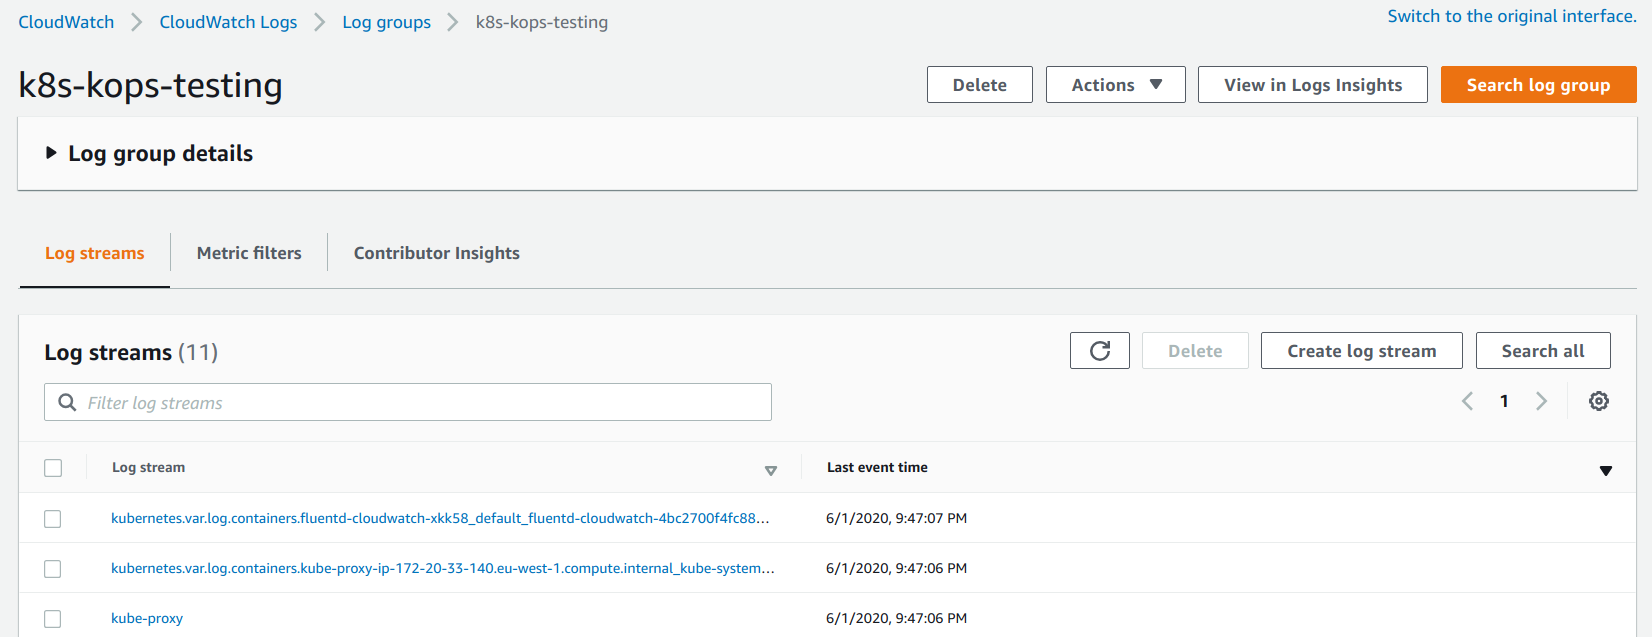
\includegraphics[width=16cm]{figures/kops-testing-cw-logs.png}
    \captionsetup{justification=centering,margin=2cm}
    \caption{AWS CloudWatch with logs from a Kubernetes cluster}}
\end{figure}
\begin{figure}[H]
    \centering
    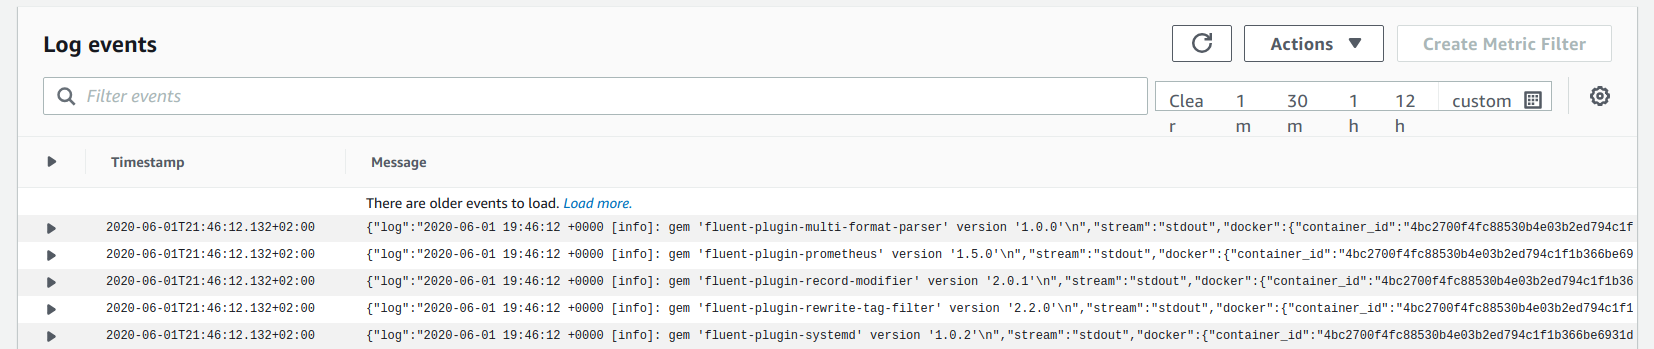
\includegraphics[width=16cm]{figures/kops-testing-cw-logs2.png}
    \captionsetup{justification=centering,margin=2cm}
    \caption{AWS CloudWatch with logs from a Kubernetes cluster}}
\end{figure}

An example log message looks like this:
\begin{lstlisting}[basicstyle=\tiny,caption={An example Kubernetes log message, presented on AWS CloudWatch},captionpos=b,language=Bash,xleftmargin=1cm]
{
    "log": "2020-06-01 19:46:12 +0000 [info]: gem 'fluent-plugin-multi-format-parser' version '1.0.0'\n",
    "stream": "stdout",
    "docker": {
        "container_id": "4bc2700f4fc88530b4e03b2ed794c1f1b366be6931d8500a8ccf21503d2c5b97"
    },
    "kubernetes": {
        "container_name": "fluentd-cloudwatch",
        "namespace_name": "default",
        "pod_name": "fluentd-cloudwatch-xkk58",
        "container_image": "fluent/fluentd-kubernetes-daemonset:v1.7.3-debian-cloudwatch-1.0",
        "container_image_id": "docker-pullable://fluent/fluentd-kubernetes-daemonset@sha256:9b8b2f99ea884853205150364eceaac9fff5ea97fc3300cc0080f48c3eac8b8a",
        "pod_id": "9fc38bd1-ff7b-4d29-9593-15796a7e5f94",
        "host": "ip-172-20-33-140.eu-west-1.compute.internal",
        "labels": {
            "app": "fluentd-cloudwatch",
            "controller-revision-hash": "68f7dc7cc",
            "pod-template-generation": "1",
            "release": "fluentd-cloudwatch"
        },
        "master_url": "https://100.64.0.1:443/api",
        "namespace_id": "4044bfd2-e836-43a1-bda1-71da0e985b9a"
    }
}
\end{lstlisting}


It can be also verified, that the custom labels applied to AWS resources by the cluster YAML configuration file, are indeed visible. The custom label here is: \textit{deployment: kops-testing}.
\begin{figure}[H]
    \centering
    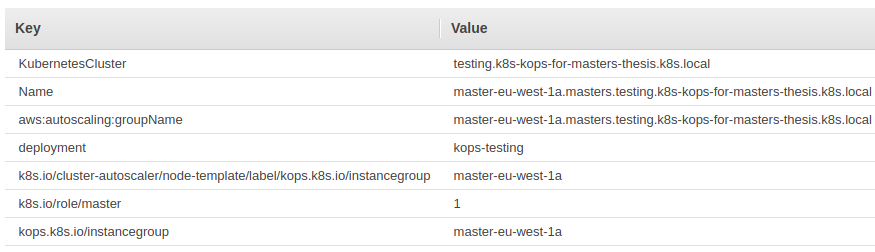
\includegraphics[width=16cm]{figures/kops-master-ec2-custom-tags.png}
    \captionsetup{justification=centering,margin=2cm}
    \caption{AWS Management Console showing tags applied on EC2 instance which is a master node}}
\end{figure}

When it comes to monitoring the cluster resources, some metrics are available by default on AWS EC2 dashboard. The information concerning CPU utilization or incoming network quantity in bytes can be viewed without any additional configuration. The example charts are depicted below.
\begin{figure}[H]
    \centering
    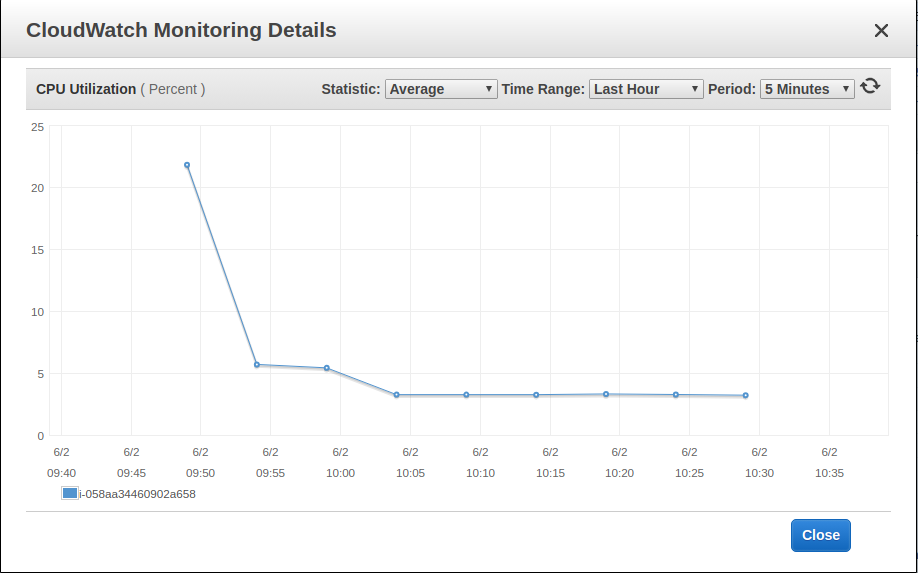
\includegraphics[width=13cm]{figures/k8s-kops-metrics-node1.png}
    \captionsetup{justification=centering,margin=2cm}
    \caption{CloudWatch metrics of a worker node, CPU utilization}}
\end{figure}
\begin{figure}[H]
    \centering
    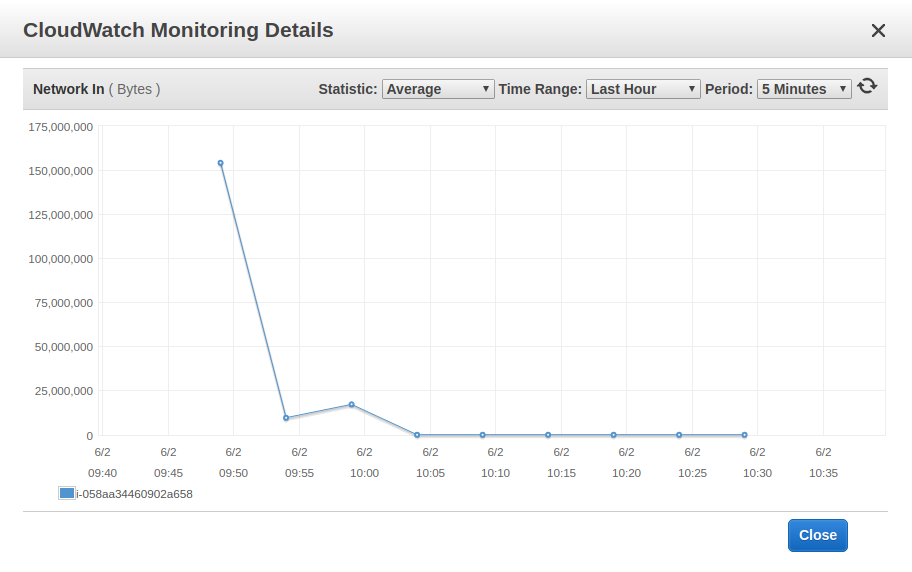
\includegraphics[width=13cm]{figures/k8s-kops-metrics-node2.png}
    \caption{CloudWatch metrics of a worker node, Network input}}
\end{figure}

When it comes to \textbf{Central Audit} requirement, no manual steps were needed. One can just log into AWS Management Console through a web browser, go to the AWS CloudTrail service and view the events history. Each event can be viewed and in return, information in JSON format is received. A table with events is presented on the picture below.

\begin{figure}[H]
    \centering
    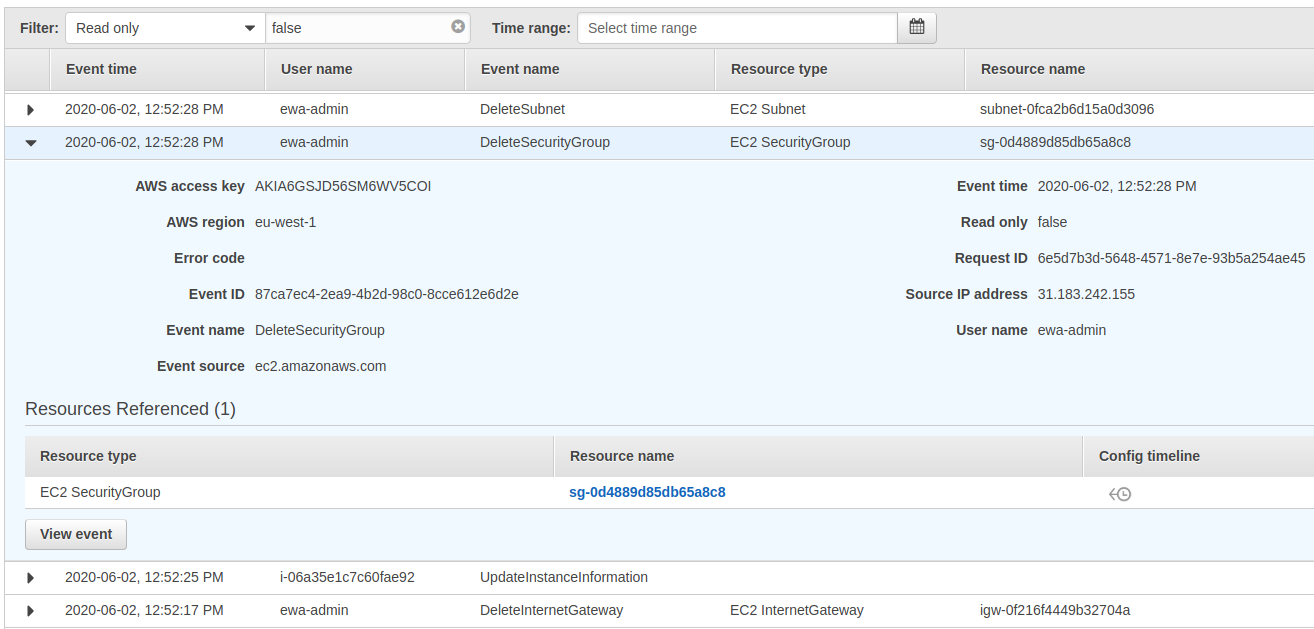
\includegraphics[width=13cm]{figures/kops-cloudtrail.png}
    \captionsetup{justification=centering,margin=2cm}
    \caption{CloudTrail events of a kops cluster}}
\end{figure}

The next operation is to backup a cluster namespace. Velero was chosen as an application to facilitate backup. In order to install Velero CLI, one can run:
\begin{lstlisting}[basicstyle=\tiny,caption={Automated command to install Velero CLI},captionpos=b,language=Bash,xleftmargin=1cm]
kops$ ./tasks _install_velero_cli
\end{lstlisting}

The above command installed Velero client. A Velero Server must be also deployed on a Kubernetes cluster. Before it is done, AWS IAM user must be created and proper permissions must be assigned to it. The instructions how to deal with AWS IAM for Velero were available at Github\cite{velero-aws-plugin}. In order to be able to repeat the steps easily, all the instructions were saved to a Bash script as: \textit{src/velero/generate-velero-credentials.sh}. Running it should result in generating two credentials and generating a file called \textit{credentials-velero} in the current directory. The file had such contents:
\begin{lstlisting}[basicstyle=\tiny,caption={Contents of AWS credentials file}]
[default]
aws_access_key_id=<REPLACE-ME-WITH-SECRET>
aws_secret_access_key=<REPLACE-ME-WITH-SECRET>
\end{lstlisting}

Afterwards, a Velero Server was deployed, using a Helm chart. The following command was used:

\begin{lstlisting}[basicstyle=\tiny,caption={Deploying a Velero Helm chart},captionpos=b,language=Bash,xleftmargin=1cm]
$ kubectl create namespace velero
$ helm repo add vmware-tanzu https://vmware-tanzu.github.io/helm-charts
$ helm install velero --namespace velero -f ${PWD}/../velero/velero-chart-values.yaml \
--set configuration.backupStorageLocation.bucket=${K8S_EXP_VELERO_S3_BUCKET} \
--set configuration.backupStorageLocation.prefix=${K8S_EXP_ENVIRONMENT} \
--set configuration.backupStorageLocation.config.region=${K8S_EXP_REGION} \
--set-file credentials.secretContents.cloud=credentials-velero \
--wait --atomic vmware-tanzu/velero
\end{lstlisting}

Then, a backup location for Velero was configured. It was done with the following command:
\begin{lstlisting}[basicstyle=\tiny,caption={Choosing a backup storage location for Velero}]
$ velero backup-location create default \
  --provider aws \
  --bucket ${K8S_EXP_VELERO_S3_BUCKET} \
  --prefix ${K8S_EXP_ENVIRONMENT} \
  --config region=${K8S_EXP_REGION}
Backup storage location "default" configured successfully.
\end{lstlisting}

And then, finally, the steps from Velero documentation was followed\cite{velero-examples}. A test application (provided by Velero) was deployed and backuped. The test application was deployed to a Kubernetes namespace: \textit{nginx-example}.   It was verified also that the Kubernetes resources were created.
\begin{lstlisting}[basicstyle=\tiny,caption={Testing backup operation}]
$ kubectl apply -f ../velero/velero-example.yaml
namespace/nginx-example created
deployment.apps/nginx-deployment created
service/my-nginx created
$ kubectl get -n nginx-example all
NAME                                    READY   STATUS              RESTARTS   AGE
pod/nginx-deployment-7cd5ddccc7-9drfn   1/1     Running   0          26s
pod/nginx-deployment-7cd5ddccc7-hr9zg   1/1     Running             0          7s

NAME               TYPE           CLUSTER-IP      EXTERNAL-IP        PORT(S)        AGE
service/my-nginx   LoadBalancer   100.64.170.74   a64fbc3f7b55c45aead4f113025d8a34-1346547608.eu-west-1.elb.amazonaws.com   \
80:31927/TCP   7s

NAME                               READY   UP-TO-DATE   AVAILABLE   AGE
deployment.apps/nginx-deployment   1/2     2            1           7s

NAME                                          DESIRED   CURRENT   READY   AGE
replicaset.apps/nginx-deployment-7cd5ddccc7   2         2         1       8s
$ velero backup create nginx-backup1 --include-namespaces nginx-example
Backup request "nginx-backup1" submitted successfully.
Run `velero backup describe nginx-backup1` or `velero backup logs nginx-backup1` for more details.
$ velero backup describe nginx-backup1
Name:         nginx-backup1
# output partially ommitted
Phase:  Completed
$ velero backup logs nginx-backup1
# output partially ommitted
time="2020-06-03T13:35:51Z" level=info msg="Backed up a total of 24 items" \
backup=velero/nginx-backup1 logSource="pkg/backup/backup.go:436" progress=
\end{lstlisting}

The backup result was stored in an S3 bucket and it is presented in the image below:
\begin{figure}[H]
    \centering
    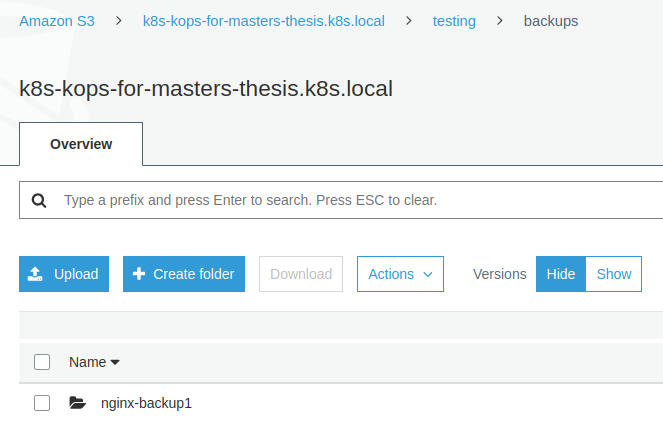
\includegraphics[width=10cm]{figures/kops-velero-backup.png}
    \captionsetup{justification=centering,margin=2cm}
    \caption{Backup of a Kubernetes namespace created by Velero, kept in an S3 bucket}}
\end{figure}

Next, a disaster was simulated. The whole \textit{nginx-example} namespace was deleted:
\begin{lstlisting}[basicstyle=\tiny,caption={Simulating a disaster to test backup}]
$ kubectl delete namespaces nginx-example
namespace "nginx-example" deleted
$ kubectl get -n nginx-example all
No resources found in nginx-example namespace.
\end{lstlisting}

The last step was to restore the namespace from Velero backup. It was successful.
\begin{lstlisting}[basicstyle=\tiny,caption={Restoring the backup}]
$ velero restore create --from-backup nginx-backup1
Restore request "nginx-backup1-20200603133811" submitted successfully.
Run `velero restore describe nginx-backup1-20200603133811` or \
  `velero restore logs nginx-backup1-20200603133811` for more details.
$ kubectl get -n nginx-example all
NAME                                    READY   STATUS    RESTARTS   AGE
pod/nginx-deployment-7cd5ddccc7-9drfn   1/1     Running   0          9s
pod/nginx-deployment-7cd5ddccc7-hr9zg   1/1     Running   0          8s

NAME               TYPE           CLUSTER-IP      EXTERNAL-IP   PORT(S)     AGE
service/my-nginx   LoadBalancer   100.71.21.114   \
abf6080d1d43a43ba97999bb6b22cabc-2114878664.eu-west-1.elb.amazonaws.com   80:32539/TCP   8s

NAME                               READY   UP-TO-DATE   AVAILABLE   AGE
deployment.apps/nginx-deployment   2/2     2            2           8s

NAME                                          DESIRED   CURRENT   READY   AGE
replicaset.apps/nginx-deployment-7cd5ddccc7   2         2         2       8s
\end{lstlisting}


Then, autoscaling was tested. The autoscaler Kubernetes resources were deployed with:
\begin{lstlisting}[basicstyle=\tiny,caption={Bash command to deploy autoscaker}]
kops$ ./tasks _enable_as
\end{lstlisting}
which basically just deployed the resources configured at autoscaler git repository\cite{as-github}. Some modifications were also applied to the cluster YAML configuration, namely: under \textit{additionalPolicies} of node configuration, the following code was added:
\begin{lstlisting}[basicstyle=\tiny,caption={IAM Policies needed by autoscaler}]
{
  "Effect": "Allow",
  "Action": [
    "autoscaling:DescribeAutoScalingGroups",
    "autoscaling:DescribeAutoScalingInstances",
    "autoscaling:DescribeLaunchConfigurations",
    "autoscaling:SetDesiredCapacity",
    "autoscaling:TerminateInstanceInAutoScalingGroup",
    "autoscaling:DescribeTags"
  ],
  "Resource": "*"
}
\end{lstlisting}
Also, additional labels for InstanceGroup of worker nodes were set and maximum number of worker nodes were set to 2. This went smoothly thanks to a blog post\cite{as-blog}. The modified configuration is presented below:
\begin{lstlisting}[basicstyle=\tiny,caption={Kops cluster YAML configuration needed for autoscaler}]
spec:
  cloudLabels:
    service: k8s_node
    k8s.io/cluster-autoscaler/enabled: ""
    k8s.io/cluster-autoscaler/testing.k8s-kops-for-masters-thesis.k8s.local: ""
  minSize: 1
  maxSize: 2
\end{lstlisting}

In order to test the autoscaling, a test application was deployed with:
\begin{lstlisting}[basicstyle=\tiny,caption={Deploying a test application},captionpos=b,language=Bash,xleftmargin=1cm]
tests$ ./deploy-test-service.sh
\end{lstlisting}
After the above command ended with success, it was verified that 1 pod replica was deployed. Since, the task here was to make the autoscaler decide to scale out - to add another node, the test application deployment was scaled, so that 200 pod replicas were deployed.
\begin{lstlisting}[basicstyle=\tiny,caption={Scaling the test application pod replicas},captionpos=b,language=Bash,xleftmargin=1cm]
kops$ kubectl get -n testing deployment
NAME             READY   UP-TO-DATE   AVAILABLE   AGE
apache-testing   1/1     1            1           9m48s
kops$ kubectl scale -n testing deployment apache-testing --replicas=200
deployment.apps/apache-testing scaled
kops$ kubectl get -n testing deployment
NAME             READY    UP-TO-DATE   AVAILABLE   AGE
apache-testing   12/200   200          12        13m
\end{lstlisting}
This triggered the creation of another node and in a short while, there were two nodes in the cluster:
\begin{lstlisting}[basicstyle=\tiny,caption={Listing the EC2 instances, 1 of them was created by autoscaler}]
kops$ aws ec2 describe-instances --filters "Name=tag-key,Values=deployment" \
  --query "Reservations[*].Instances[*].{PublicIP:PublicIpAddress,Name:Tags[?Key=='Name']|[0].Value,Status:State.Name}"
[
    [
        {
            "PublicIP": "34.242.4.10",
            "Name": "master-eu-west-1a.masters.testing.k8s-kops-for-masters-thesis.k8s.local",
            "Status": "running"
        }
    ],
    [
        {
            "PublicIP": "34.247.37.124",
            "Name": "nodes.testing.k8s-kops-for-masters-thesis.k8s.local",
            "Status": "running"
        }
    ],
    [
        {
            "PublicIP": "3.249.123.18",
            "Name": "nodes.testing.k8s-kops-for-masters-thesis.k8s.local",
            "Status": "running"
        }
    ]
]
\end{lstlisting}
Afterwards, the pod replicas were scaled back to 1 and then, autoscaler terminated one of the worker nodes. Soon, one of the EC2 instances was in the status: terminated. This proved that autoscaler works for a Kubernetes cluster deployed with kops.

When it comes to running a cluster in the High Availability mode, there were no problems whatsoever. No matter if the cluster was created with one master node or multiple master nodes - it was working. In HA mode, the following was returned as information about the cluster:
\begin{lstlisting}[basicstyle=\tiny,caption={Getting information about the cluster}]
$ kubectl get nodes
NAME                                          STATUS   ROLES    AGE   VERSION
ip-172-20-108-29.eu-west-1.compute.internal   Ready    master   73s   v1.16.9
ip-172-20-55-72.eu-west-1.compute.internal    Ready    node     49s   v1.16.9
ip-172-20-61-242.eu-west-1.compute.internal   Ready    master   74s   v1.16.9
ip-172-20-89-96.eu-west-1.compute.internal    Ready    master   75s   v1.16.9
$ kops validate
Validating cluster testing.k8s-kops-for-masters-thesis.k8s.local

INSTANCE GROUPS
NAME			ROLE	MACHINETYPE	MIN	MAX	SUBNETS
master-eu-west-1a	Master	t2.micro	1	1	eu-west-1a
master-eu-west-1b	Master	t2.micro	1	1	eu-west-1b
master-eu-west-1c	Master	t2.micro	1	1	eu-west-1c
nodes			Node	t2.micro	1	1	eu-west-1a

NODE STATUS
NAME						ROLE	READY
ip-172-20-108-29.eu-west-1.compute.internal	master	True
ip-172-20-55-72.eu-west-1.compute.internal	node	True
ip-172-20-61-242.eu-west-1.compute.internal	master	True
ip-172-20-89-96.eu-west-1.compute.internal	master	True

Your cluster testing.k8s-kops-for-masters-thesis.k8s.local is ready
\end{lstlisting}

The machines can be also viewed on AWS Management Console:
\begin{figure}[H]
    \centering
    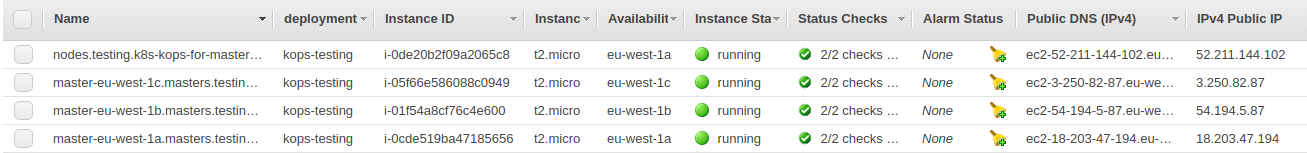
\includegraphics[width=18cm]{figures/k8s-kops-ha-aws.png}
    \captionsetup{justification=centering,margin=2cm}
    \caption{EC2 instance in HA mode for kops cluster}}
\end{figure}

Also, the tests were invoked both in HA mode and also with one master cluster. The tests succeeded in both cases. In HA mode, all the Kubernetes control plane components were duplicated (in this case - three times):
\begin{lstlisting}[basicstyle=\tiny,caption={Kubernetes control plane components, HA}]
$ kubectl -n kube-system get pod
NAME                                                                  READY   STATUS    RESTARTS   AGE
dns-controller-776cdf4ff4-xw4tg                                       1/1     Running   0          2m18s
etcd-manager-events-ip-172-20-108-29.eu-west-1.compute.internal       1/1     Running   0          66s
etcd-manager-events-ip-172-20-61-242.eu-west-1.compute.internal       1/1     Running   0          86s
etcd-manager-events-ip-172-20-89-96.eu-west-1.compute.internal        1/1     Running   0          96s
etcd-manager-main-ip-172-20-108-29.eu-west-1.compute.internal         1/1     Running   0          53s
etcd-manager-main-ip-172-20-61-242.eu-west-1.compute.internal         1/1     Running   0          56s
etcd-manager-main-ip-172-20-89-96.eu-west-1.compute.internal          1/1     Running   0          80s
kops-controller-2tz4h                                                 1/1     Running   0          2m8s
kops-controller-7mr7s                                                 1/1     Running   0          2m14s
kops-controller-psfch                                                 1/1     Running   0          2m8s
kube-apiserver-ip-172-20-108-29.eu-west-1.compute.internal            1/1     Running   3          110s
kube-apiserver-ip-172-20-61-242.eu-west-1.compute.internal            1/1     Running   3          114s
kube-apiserver-ip-172-20-89-96.eu-west-1.compute.internal             1/1     Running   3          92s
kube-controller-manager-ip-172-20-108-29.eu-west-1.compute.internal   1/1     Running   0          2m6s
kube-controller-manager-ip-172-20-61-242.eu-west-1.compute.internal   1/1     Running   0          105s
kube-controller-manager-ip-172-20-89-96.eu-west-1.compute.internal    1/1     Running   0          79s
kube-dns-autoscaler-594dcb44b5-ccnjf                                  1/1     Running   0          2m19s
kube-dns-b84c667f4-5tb9z                                              3/3     Running   0          105s
kube-dns-b84c667f4-8vmh4                                              3/3     Running   0          2m21s
kube-proxy-ip-172-20-108-29.eu-west-1.compute.internal                1/1     Running   0          116s
kube-proxy-ip-172-20-55-72.eu-west-1.compute.internal                 1/1     Running   0          110s
kube-proxy-ip-172-20-61-242.eu-west-1.compute.internal                1/1     Running   0          65s
kube-proxy-ip-172-20-89-96.eu-west-1.compute.internal                 1/1     Running   0          61s
kube-scheduler-ip-172-20-108-29.eu-west-1.compute.internal            1/1     Running   0          2m
kube-scheduler-ip-172-20-61-242.eu-west-1.compute.internal            1/1     Running   0          2m13s
kube-scheduler-ip-172-20-89-96.eu-west-1.compute.internal             1/1     Running   0          112s
\end{lstlisting}

\subsubsection{Testing a cluster}
\label{kops-testing}
All the tests can be invoked with a single command:
\begin{lstlisting}[basicstyle=\tiny,caption={Testing a kops cluster}]
kops$ ./tasks _test
\end{lstlisting}

This one command runs the following:
\begin{lstlisting}[basicstyle=\tiny,caption={Testing a kops cluster - deeper dive}]
$ set -x
$ time kops validate cluster ${K8S_EXP_CLUSTER_NAME} --state "s3://${K8S_EXP_KOPS_S3_BUCKET}"
$ cd ../tests
$ time bats tests.bats
$ cd ../kops
\end{lstlisting}

The \textit{kops validate cluster} command is provided by the kops CLI. It checks that all k8s master and worker nodes are running and have "Ready" status, that all the components are healthy and that all pods in the kube-system namespace are running and healthy\cite{online-kops-valid}. The next command runs the Bats-core tests. They test the version of Kubernetes, number of worker nodes and also they deploy a test Helm chart with Apache Server. All the tests and the deployment (and later deletion) of the Apache Helm chart are automated and intended to be idempotent. Thanks to such a test, it is verified that such a Kubernetes cluster is ready to use for the end users.

The test Apache Server serves a very simple website, which all code is just one index.html file with the following contents:
\begin{lstlisting}[basicstyle=\tiny,caption={Contents of a test application - Apache web server}]
<html>
<head>
<title>Hello world</title>
</head>
<body>
<p>Welcome to my Master Thesis website!</p>
</body>
</html>
\end{lstlisting}
Thus, there is a test that runs: \textit{curl} command and expects that the output contains "Welcome to my Master Thesis website!". Such a test is possible thanks to an ingress resource provided by the Apache Helm Chart. When this ingress is deployed on a Kubernetes cluster on AWS, an Elastic Load Balancer (ELB) is created. ELB is an AWS resource. The ELB provides us with the endpoint that can be used with \textit{curl}.

The tests were run with Bats-core and their code is presented below:
\begin{lstlisting}[basicstyle=\tiny,caption={Bats-core tests}]
@test "kubernetes machines have correct version" {
  run /bin/bash -c "kubectl version | grep 'Server Version'"
  # this is printed on test failure only
  echo "# test cmd output: $output"
  [[ "${output}" =~ "v1.16" ]]
  [ "$status" -eq 0 ]
}

@test "1 kubernetes worker nodes have status: Ready" {
  run /bin/bash -c "chmod +x get-workers-count.sh && ./get-workers-count.sh"
  # this is printed on test failure only
  echo "# test cmd output: $output"
  [[ "${output}" =~ "1" ]]
  [ "$status" -eq 0 ]
}

@test "kubectl cluster-info returns expected output" {
  run /bin/bash -c "kubectl cluster-info"
  # this is printed on test failure only
  echo "# test cmd output: $output"
  [[ "${output}" =~ "Kubernetes master" ]]
  [[ "${output}" =~ "https://" ]]
  # this works for kops cluster only:
  # [[ "${output}" =~ "https://api-testing-k8s-kops-for" ]]
  # output for eks:
  # Kubernetes master is running at https://E1B139B821FFAEF37082A7B64BB951FC.gr7.eu-west-1.eks.amazonaws.com
  # CoreDNS is running at https://E1B139B821FFAEF37082A7B64BB951FC.gr7.eu-west-1.eks.amazonaws.com/api/v1/namespaces/kube-system/services/kube-dns:dns/proxy
  [ "$status" -eq 0 ]
}

@test "a test application can be deployed on kubernetes" {
  run /bin/bash -c "chmod +x ./deploy-test-service.sh && ./deploy-test-service.sh"
  # this is printed on test failure only
  echo "# test cmd output: $output"
  [[ "${output}" =~ "Success" ]]
  [ "$status" -eq 0 ]

  # k8s resource: pod was created
  run /bin/bash -c "kubectl get --namespace=testing pods"
  # this is printed on test failure only
  echo "# test cmd output: $output"
  [[ "${output}" =~ "apache-testing" ]]
  [[ "${output}" =~ "Running" ]]
  [ "$status" -eq 0 ]

  # k8s resource: svc was created
  run /bin/bash -c "kubectl get --namespace=testing svc"
  # this is printed on test failure only
  echo "# test cmd output: $output"
  [[ "${output}" =~ "apache-testing" ]]
  [ "$status" -eq 0 ]

  # k8s resource: ing was created
  run /bin/bash -c "kubectl get --namespace=testing ing"
  # this is printed on test failure only
  echo "# test cmd output: $output"
  [[ "${output}" =~ "apache-testing" ]]
  [ "$status" -eq 0 ]
}

@test "a test application is available (ingress resource works)" {
  # the LoadBalancer on AWS does not work right away, so here
  # we try it many times, until it works (max 400 trials)
  run /bin/bash -c "export SERVICE_IP=$(kubectl get svc --namespace testing apache-testing --template '{{ range (index .status.loadBalancer.ingress 0) }}{{.}}{{ end }}') && chmod +x test-timeout-until.sh && ./test-timeout-until.sh \"curl --max-time 2 -L http://\$SERVICE_IP 2>/dev/null | grep 'Welcome to my Master Thesis website'\" \"400\" \"curl --max-time 2 -L http://\$SERVICE_IP 2>/dev/null | grep 'Welcome to my Master Thesis website'\""
  # this is printed on test failure only
  echo "# test cmd output: $output"
  [[ "${output}" =~ "Welcome to my Master Thesis website" ]]
  [ "$status" -eq 0 ]
}

@test "a test service (test website) can be deleted from kubernetes" {
  run /bin/bash -c 'helm uninstall --namespace="testing" "apache-testing" && kubectl delete -f config-map-www-contents.yaml && kubectl delete namespace "testing"'
  echo "# test cmd output: $output"
  [[ "${output}" =~ "uninstalled" ]]
  [ "$status" -eq 0 ]

  # pod, svc and ing resources were deleted
  run /bin/bash -c 'kubectl get --namespace=testing pods,svc,ing'
  echo "# test cmd output: $output"
  [[ "${output}" =~ "No resources found in testing namespace" ]]
  [ "$status" -eq 0 ]
}
\end{lstlisting}
Several helpful scripts were created and used for the tests. All the needed files are put in the git repository on Github.com.

%%%

\subsubsection{Deleting a cluster}

Deleting a cluster was fully automated and performed with:

\begin{lstlisting}[basicstyle=\tiny,caption={Testing a kops cluster}]
kops$ ./tasks _delete
\end{lstlisting}

\subsubsection{Troubleshooting}
\label{kops-troubleshooting}

\textbf{The first problem} was, that the command responsible for creating a cluster did not wait until the cluster was ready. It returned as soon as the AWS resources were scheduled for creation. This was a problem, because if one wanted to create, test and then delete a Kubernetes cluster in a CI pipeline, then the tests would never work. And the pipeline would always fail. The solution for this problem was already described in the section \ref{kops-creating-the-cluster}.

\textbf{The second problem} was how to configure logging to AWS CloudWatch. The documentation of the Helm chart: kube2iam\cite{kube2iam} provided an example command of how to deploy the chart: \textit{helm install stable/kube2iam --name my-release}. But this resulted in errors, which are presented below, thanks to debugging the kube2iam pod.
\begin{lstlisting}[basicstyle=\tiny,caption={Debugging kube2iam pod},captionpos=b,language=Bash,xleftmargin=1cm]
$ kubectl get pod
NAME                       READY   STATUS             RESTARTS   AGE
kube2iam-2c8vv             0/1     CrashLoopBackOff   9          17m
$ kubectl logs kube2iam-2c8vv
E0601 10:35:53.142224       1 reflector.go:199] github.com/jtblin/kube2iam/vendor/k8s.io/client-go/tools/cache/reflector.go:94: Failed to list *v1.Pod: pods is forbidden: User "system:serviceaccount:default:default" cannot list resource "pods" in API group "" at the cluster scope
E0601 10:35:53.142621       1 reflector.go:199] github.com/jtblin/kube2iam/vendor/k8s.io/client-go/tools/cache/reflector.go:94: Failed to list *v1.Namespace: namespaces is forbidden: User "system:serviceaccount:default:default" cannot list resource "namespaces" in API group "" at the cluster scope
\end{lstlisting}

These errors went away, when the chart was deployed with additional settings set: \textit{helm upgrade "kube2iam" --namespace="default" --wait --atomic --set rbac.create=true stable/kube2iam}.

\textbf{The third problem} concerned the lack of permissions of the fluentd-cloudwatch pod. It manifested in the following way:
\begin{lstlisting}[basicstyle=\tiny,caption={Debugging the fluent-cloudwatch pod},captionpos=b,language=Bash,xleftmargin=1cm]
$ kubectl logs fluentd-cloudwatch-xkk58
2020-06-01 11:03:14 +0000 [warn]: #0 [out_cloudwatch_logs_host_logs] failed to flush the buffer. retry_time=8 next_retry_seconds=2020-06-01 11:05:22 +0000 chunk="5a703b5e45c9592f24399f9b73acaf43" error_class=Aws::CloudWatchLogs::Errors::AccessDeniedException error="User: arn:aws:sts::976184668068:assumed-role/nodes.testing.k8s-kops-for-masters-thesis.k8s.local/i-04a926040234f36d6 is not authorized to perform: logs:DescribeLogGroups on resource: arn:aws:logs:eu-west-1:976184668068:log-group::log-stream:"
\end{lstlisting}
This problem was also already dealt with in the section \ref{kops-creating-the-cluster}. The solution was to add IAM permissions in the YAML template configuration file. The solution was inspired by a Tobias Sturm's blog post\cite{kops-logs-cw-tobias} and by the kops documentation\cite{online-kops-iam}.

\textbf{The fourth problem} was with testing the Apache Server. The essential thing to know is that it takes some time (around 5 minutes) for the ELB to be usable by end users and thus the tests may fail in the meantime. The solution was to implement such a command that verifies the Apache Server endpoint many times, but has a maximum number of trials.

There were also \textbf{problems with deploying Velero}. For example, using the example deployment command provided on the Velero Helm Chart page on Github.com vmware-tanzu\cite{velero-helm-chart}, but omitting the aws plugin for Velero resulted in error.

\begin{lstlisting}[basicstyle=\tiny,caption={Installing Velero server},captionpos=b,language=Bash,xleftmargin=1cm]
$ helm repo add vmware-tanzu https://vmware-tanzu.github.io/helm-charts
# output omitted
$ helm install velero --namespace default \
  --set configuration.provider=aws \
  --set configuration.backupStorageLocation.name=aws \
  --set configuration.backupStorageLocation.bucket=${K8S_EXP_KOPS_S3_BUCKET} \
  --set configuration.backupStorageLocation.prefix=${K8S_EXP_ENVIRONMENT} \
  --set configuration.backupStorageLocation.config.region=${K8S_EXP_REGION} \
  --wait --atomic \
  vmware-tanzu/velero
# output omitted
$ kubectl logs -n default velero-7f476777f6-f9qlc
An error occurred: some backup storage locations are invalid: error getting backup store for location "aws": unable to locate ObjectStore plugin named velero.io/aws
\end{lstlisting}

Tinkering with that command resulted also in different error:
\begin{lstlisting}[basicstyle=\tiny,caption={Velero server installation error},captionpos=b,language=Bash,xleftmargin=1cm]
Error: release velero failed, and has been uninstalled due to atomic being set: timed out waiting for the condition
\end{lstlisting}

It was then decided to try another command to install Velero server. It pushed the progress further and revealed the problem:
\begin{lstlisting}[basicstyle=\tiny,caption={Another attempt to deploy Velero server},captionpos=b,language=Bash,xleftmargin=1cm]
$  velero install \
    --provider velero.io/aws \
    --bucket ${K8S_EXP_KOPS_S3_BUCKET} \
    --plugins velero/velero-plugin-for-aws:v1.1.0 \
    --backup-location-config s3Url=${K8S_EXP_KOPS_S3_BUCKET},region=${K8S_EXP_REGION} \
    --use-volume-snapshots=false \
    --secret-file=${PWD}/credentials-velero
Velero is installed! ⛵ Use 'kubectl logs deployment/velero -n velero' to view the status.
$ kubectl get -n velero all
NAME                          READY   STATUS    RESTARTS   AGE
pod/velero-5f8889f694-6xd7t   0/1     Pending   0          2m30s

NAME                     READY   UP-TO-DATE   AVAILABLE   AGE
deployment.apps/velero   0/1     1            0           2m30s

NAME                                DESIRED   CURRENT   READY   AGE
replicaset.apps/velero-5f8889f694   1         1         0       2m30s
$ kubectl -n velero describe pods
Name:           velero-5f8889f694-6xd7t
Namespace:      velero
Limits:
     cpu:     1
     memory:  256Mi
   Requests:
     cpu:     500m
     memory:  128Mi
Warning  FailedScheduling  70s (x5 over 6m46s)  default-scheduler  0/2 nodes are available: 2 Insufficient cpu.
\end{lstlisting}

The problem was that the Velero pod was in status: Pending. The Kubernetes documentation on pods troubleshooting suggests, that when a pod is in status: Pending, then there may be not enough resources in the cluster\cite{k8s-deb}. That was the problem in this case. The solution was to use bigger AWS instance types for node: \textit{t2.medium} instead of: \textit{t2.micro}.

Furthermore, it may be helpful to know, that whenever such error occurs, concerning the velero pod:
\begin{lstlisting}[basicstyle=\tiny,caption={Debuggin Velero},captionpos=b,language=Bash,xleftmargin=1cm]
$ kubectl get pod -n velero
NAME                      READY   STATUS             RESTARTS   AGE
velero-6fffc8dc85-cm4lb   0/1     CrashLoopBackOff   3          107s
$ kubectl logs -n velero velero-6fffc8dc85-cm4lb
An error occurred: some backup storage locations are invalid: backup store for location "aws" is invalid: rpc error: code = Unknown desc = AccessDenied: Access Denied
	status code: 403, request id: 9513047CEEBE2BD3, host id: FjQ4yAzAI1zhyFXRIS67Ww3rSqt2a1fqoeLzYEAdKsRLqx3AmpEzWWloJZXZPx9rKJs9qCH1yHY=
\end{lstlisting}
Then, it is due to invalid credentials file. It should be possible to list access keys of AWS IAM user created for velero. This can be tested with the following command:
\begin{lstlisting}[basicstyle=\tiny,caption={Listing AWS IAM keys},captionpos=b,language=Bash,xleftmargin=1cm]
$ aws iam list-access-keys --user-name velero-${K8S_EXP_CLUSTER_NAME}
{
    "AccessKeyMetadata": [
        {
            "UserName": "velero-kops-testing",
            "AccessKeyId": "<REPLACE-ME>",
            "Status": "Active",
            "CreateDate": "2020-06-03T10:22:46+00:00"
        }
    ]
}
\end{lstlisting}

A \textbf{problem considering autoscaler deployment} was observed. The Kubernetes resources provided by the official git repository on Github.com had a minor mistake. The autoscaler pod was in error state and it returned the following error:
\begin{lstlisting}[basicstyle=\tiny,caption={Debugging autoscaler},captionpos=b,language=Bash,xleftmargin=1cm]
$ kubectl describe -n kube-system pod/cluster-autoscaler-8b46dddf5-8xkns
Warning  Failed     26s                kubelet, ip-172-20-62-245.eu-west-1.compute.internal  Error: failed to start container "cluster-autoscaler": Error response from daemon: OCI runtime create failed: container_linux.go:346: starting container process caused "process_linux.go:449: container init caused \"rootfs_linux.go:58: mounting \\\"/etc/ssl/certs/ca-bundle.crt\\\" to rootfs \\\"/var/lib/docker/overlay2/0f99e6ea6c9a9f8dedf87b977b72ecff7b56e0e6e439fcd8f9275bda3dbcabe6/merged\\\" at \\\"/var/lib/docker/overlay2/0f99e6ea6c9a9f8dedf87b977b72ecff7b56e0e6e439fcd8f9275bda3dbcabe6/merged/etc/ssl/certs/ca-certificates.crt\\\" caused \\\"not a directory\\\"\"": unknown: Are you trying to mount a directory onto a file (or vice-versa)? Check if the specified host path exists and is the expected type
Warning  BackOff    12s (x2 over 42s)  kubelet, ip-172-20-62-245.eu-west-1.compute.internal  Back-off restarting failed container
\end{lstlisting}

Fortunately, this problem was handled by a public issue and the solution was also provided there\cite{as-github-issue}. The solution was to replace a path: \textit{/etc/ssl/certs/ca-certificates.crt} with \textbf{/etc/ssl/certs/ca-bundle.crt}.

Also, running the \textit{kops create cluster} initially resulted in error:
\begin{lstlisting}[caption={Error output of \textit{kops create cluster} command}]
error building tasks: error remapping manifest addons/kops-controller.addons.k8s.io/k8s-1.16.yaml: \
error parsing yaml: error converting YAML to JSON: yaml: line 56: did not find expected alphabetic or numeric character
\end{lstlisting}

The reason for this was that the development environment had a non-numeric environment variable set. It was a password and the variable value contained asterisks (\textit{****}). After the variable was unset (with the bash command: \textit{unset}), the \textit{kops create cluster} succeeded.


\subsection{Production deployment using eksctl}
\textit{This section briefly presents all the steps performed that lead to a Kubernetes cluster deployment on the AWS cloud using eksctl. Here an attempt was made to satisfy all the production environment requirements selected in the chapter: \ref{prep-prod}.}
\\

\subsubsection{Generating the YAML configuration file}
When using eksctl, it is possible to create a cluster with \textit{eksctl create cluster} command and either with setting command line options or with using a YAML file. The latter solution was chosen. In contrast to kops, it was easier to create such YAML file by hand. Due to the fact that it was desired to automate the cluster deployment across multiple environments, it was decided that there will be one configuration file named: \textit{cluster.tmpl.yaml}. This file will contain Bash variables as some values. This file will be used as a template. Then, to create a configuration file for production environment, such commands were run:
\begin{lstlisting}[basicstyle=\tiny,caption={Creating eksctl configuration},captionpos=b,language=Bash,xleftmargin=1cm]
$ export K8S_EXP_REGION="eu-west-1"
$ export K8S_EXP_ENVIRONMENT="production"
$ export K8S_EXP_CLUSTER_NAME="eks-${K8S_EXP_ENVIRONMENT}"
$ my_ip=$(curl https://ipinfo.io/ip 2>/dev/null)
$ sed "s/\${K8S_EXP_CLUSTER_NAME}/${K8S_EXP_CLUSTER_NAME}/" cluster.tmpl.yaml > cluster1.yaml
$ sed "s/\${K8S_EXP_REGION}/${K8S_EXP_REGION}/" cluster1.yaml > cluster2.yaml
$ sed "s/\${K8S_EXP_ENVIRONMENT}/${K8S_EXP_ENVIRONMENT}/" cluster2.yaml > cluster3.yaml
$ sed "s'\${my_ip}'${my_ip}/32'" cluster3.yaml > cluster.yaml
$ rm cluster1.yaml cluster2.yaml cluster3.yaml
$ time eksctl create cluster -f cluster.yaml
\end{lstlisting}

All these commands were scripted and thanks to the automation, they can be invoked just by running:
\begin{lstlisting}[basicstyle=\tiny,caption={Creating a Kubernetes cluster with eksctl},captionpos=b,language=Bash,xleftmargin=1cm]
eks$ ./tasks _create
\end{lstlisting}
This command creates a configuration file for a particular environment and then it deploys a Kubernetes cluster. The whole \textit{cluster.tmpl.yaml} file is presented below:
\begin{lstlisting}[basicstyle=\tiny,caption={Eksctl configuration file},captionpos=b,language=Bash,xleftmargin=1cm]
apiVersion: eksctl.io/v1alpha5
kind: ClusterConfig

metadata:
  name: eks-testing
  region: eu-west-1
  version: "1.16"
  tags:
    deployment: eks-testing

cloudWatch:
  clusterLogging:
    enableTypes: ["api", "audit", "authenticator", "controllerManager", "scheduler"]

nodeGroups:
  - name: ng-1
    labels: { role: worker, cluster: eks-testing }
    instanceType: t2.nano
    desiredCapacity: 1
    ssh:
      allow: true

\end{lstlisting}

Thanks to \textit{metadata.tags} set in the YAML file, the AWS resources were labeled with a custom tag: \textit{deployment: eks-testing} or \textit{deployment: eks-production} (depending on the environment). Below there are images of a CloudFormation and EKS resource with tags, viewed on AWS Management Console.
\begin{figure}[H]
    \centering
    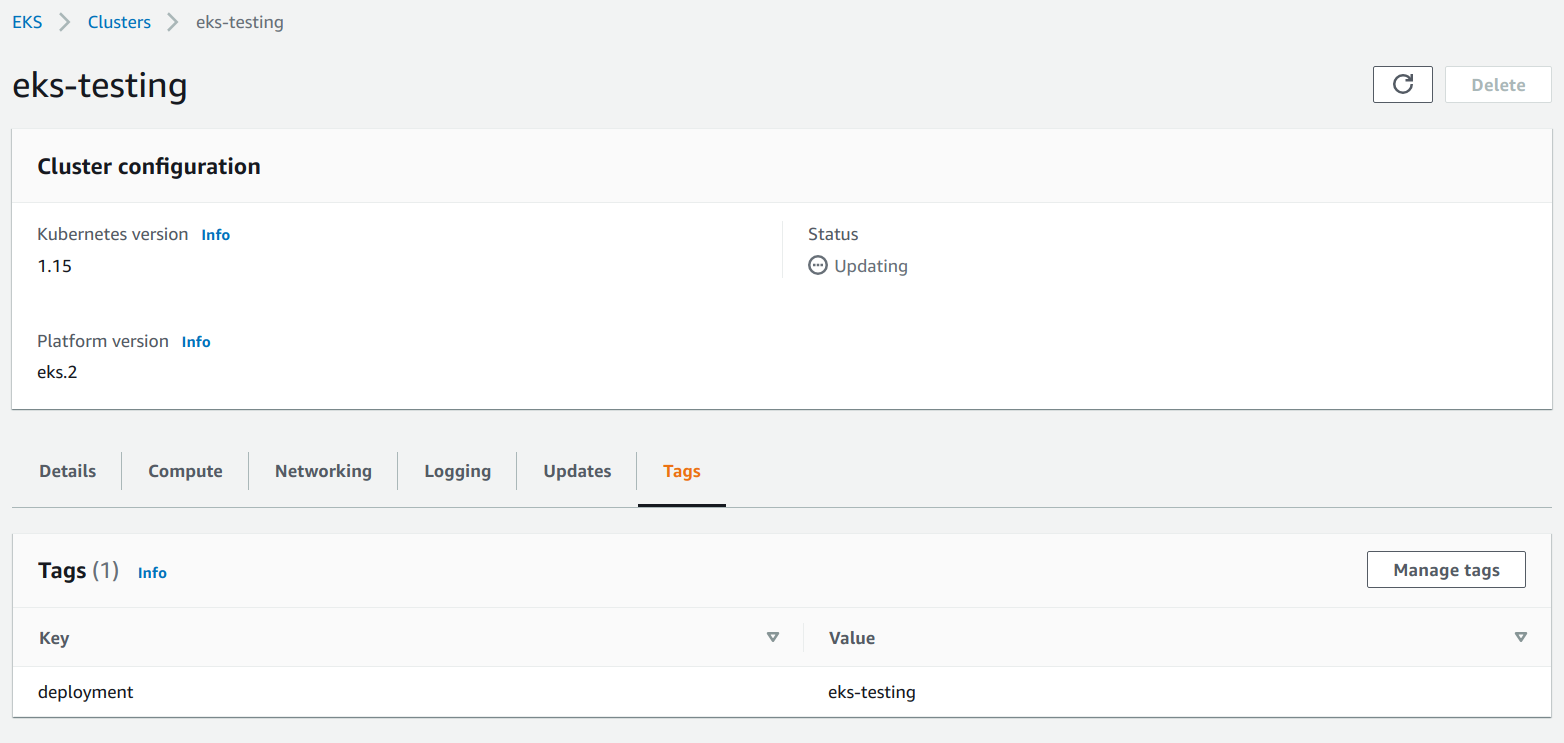
\includegraphics[width=16cm]{figures/eks-on-aws-mc-tags.png}
    \captionsetup{justification=centering,margin=2cm}
    \caption{AWS EKS resource with tags set, viewed on AWS Management Console}}
\end{figure}
\begin{figure}[H]
    \centering
    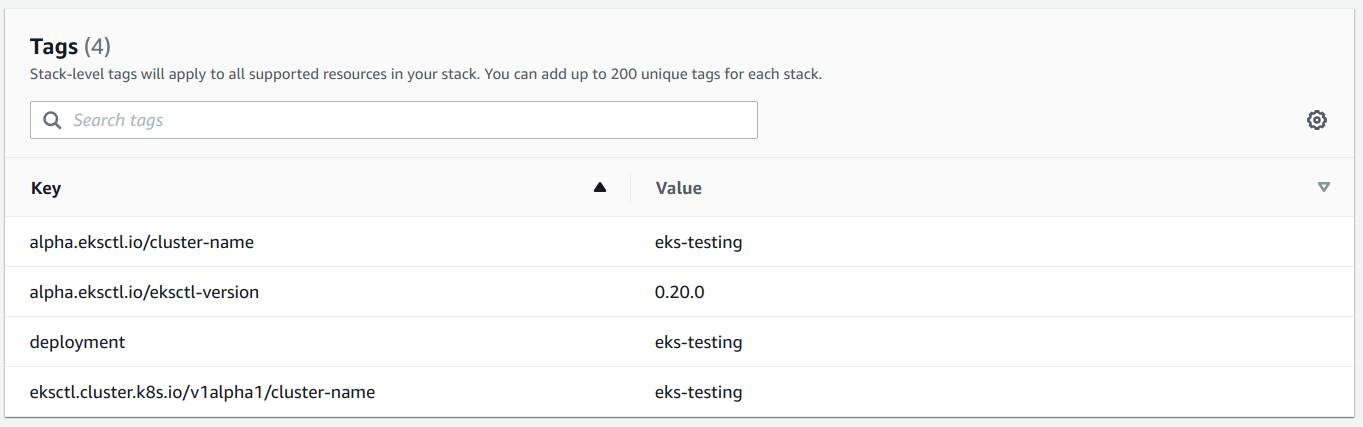
\includegraphics[width=16cm]{figures/eks-cf-tags.png}
    \captionsetup{justification=centering,margin=2cm}
    \caption{AWS CloudFormation resource with tags set, viewed on AWS Management Console}}
\end{figure}

\subsubsection{Creating a cluster}
There was one command used to generate cluster configuration (described in the previous section) and to deploy the cluster. The nice thing from the end user point of view was, that this command did not return (meaning: it waited) for the cluster to be ready. First, the control plane was deployed, then the worker nodes. For each of these two tasks (deploying control plane and deploying worker nodes) a separate CloudFormation stack was used. It was done automatically by AWS EKS. The image below presents such two stacks.

\begin{figure}[H]
    \centering
    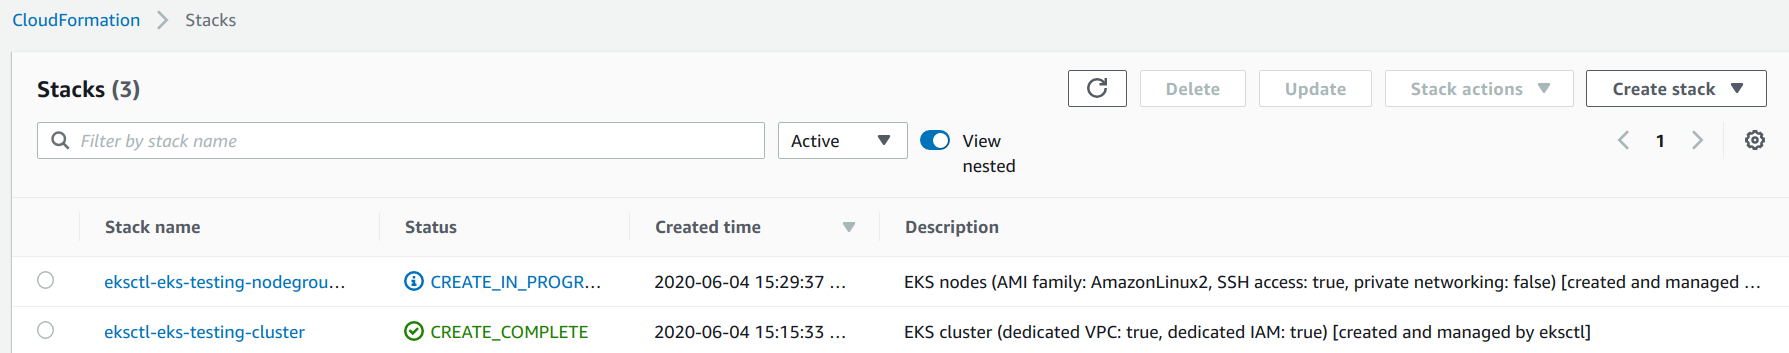
\includegraphics[width=16cm]{figures/eks-cf-stacks.png}
    \captionsetup{justification=centering,margin=2cm}
    \caption{CloudFormation stacks needed by eksctl}}
\end{figure}

It was also possible to view the AWS resources which were provided by each CloudFormation stack. It is illustrated below.
\begin{figure}[H]
    \centering
    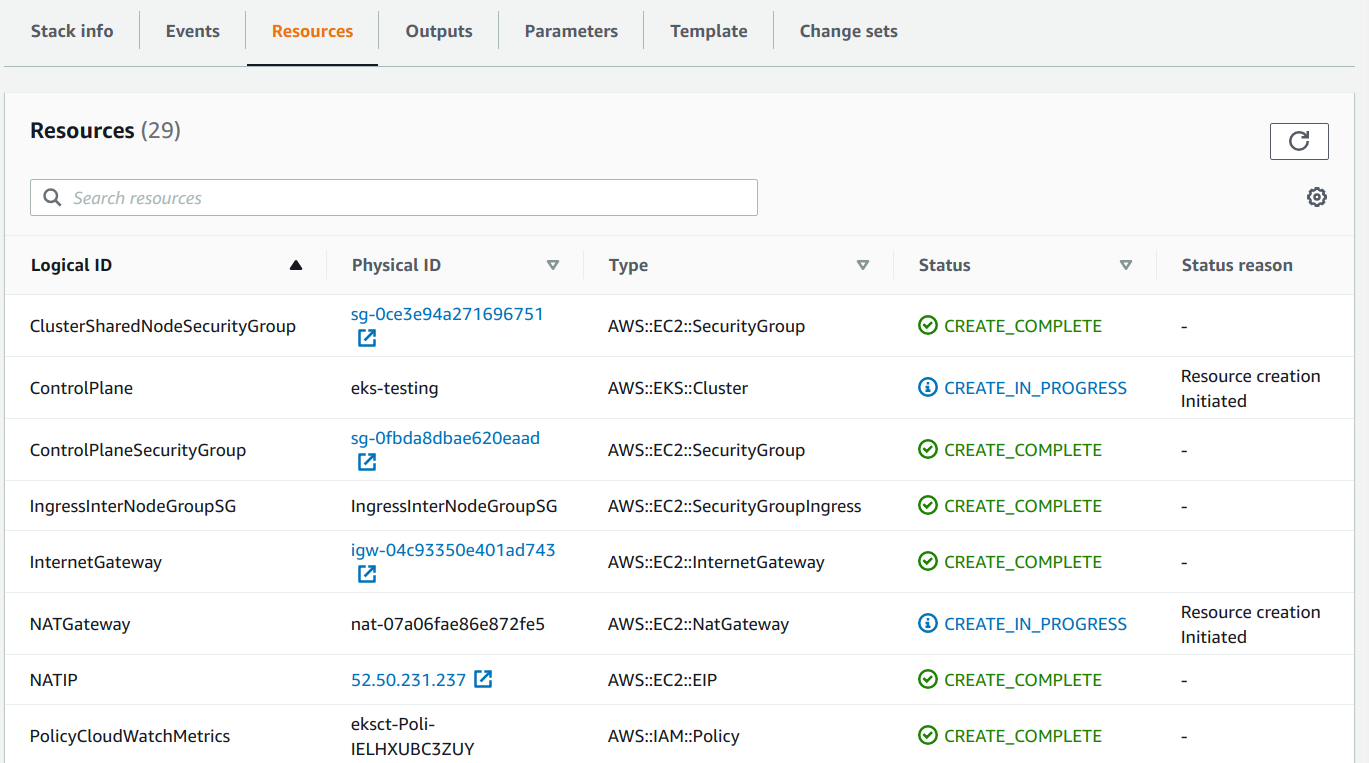
\includegraphics[width=16cm]{figures/eks-cf-resources.png}
    \captionsetup{justification=centering,margin=2cm}
    \caption{CloudFormation resources needed by eksctl}}
\end{figure}

The control plane is entirely managed by AWS and it is run across three AWS availability zones in order to ensure high availability. The end user has even no access to the control plane, meaning: there is no EC2 instance with master node visible and when listing all Kubernetes nodes, only the worker nodes are visible.
\begin{figure}[H]
    \centering
    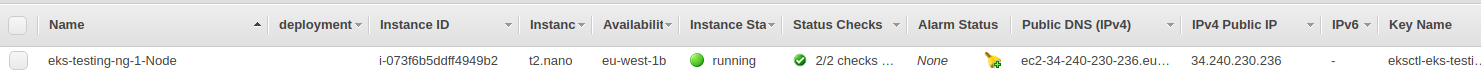
\includegraphics[width=16cm]{figures/eks-on-aws-node.png}
    \captionsetup{justification=centering,margin=2cm}
    \caption{AWS EKS instances, no master nodes}}
\end{figure}

A few sources claimed that the creation of Kubernetes cluster on AWS EKS should take 10 - 15 minutes\cite{eks-blog-part1}\cite{eks-blog2}, but in this particular case it took about 20 minutes. Also, to the best of this work’s author knowledge, there was no command which allows to reconfigure the cluster using all settings from the YAML configuration file. This means that when there was a need to change e.g. tags of the AWS resources, the cluster must have been deleted and created from scratch. An issue on Github.com was created to acknowledge this problem\cite{eksctl-no-config-update}. This cannot be achieved with eksctl, but many settings can be changed with AWS CLI, for example cluster endpoint\cite{eks-cluster-endpoint}. There is, however, a command that enables to upgrade the control plane to the next Kubernetes version (if it available). This command is:
\begin{lstlisting}[basicstyle=\tiny,caption={Updating eksctl cluster},captionpos=b,language=Bash,xleftmargin=1cm]
$ eksctl update cluster
\end{lstlisting}
And also, some particular settings may be set using \textit{eksctl utils} command. For example\cite{eksctl-net}:
\begin{lstlisting}[basicstyle=\tiny,caption={Updating eksctl cluster configuration},captionpos=b,language=Bash,xleftmargin=1cm]
$ eksctl utils set-public-access-cidrs --cluster=<cluster> 1.1.1.1/32,2.2.2.0/24
$ eksctl utils set-public-access-cidrs -f config.yaml
\end{lstlisting}


Enabling the Central Logging was very easy. All what was needed was adding the following code to the configuration YAML file:
\begin{lstlisting}[basicstyle=\tiny,caption={Enabling logging in eksctl cluster},captionpos=b,language=Bash,xleftmargin=1cm]
cloudWatch:
  clusterLogging:
    enableTypes: ["api", "audit", "authenticator", "controllerManager", "scheduler"]
\end{lstlisting}

In result, an AWS LogGroup was created and all the log messages from Kubernetes components were directed onto the LogGroup.

\begin{figure}[H]
    \centering
    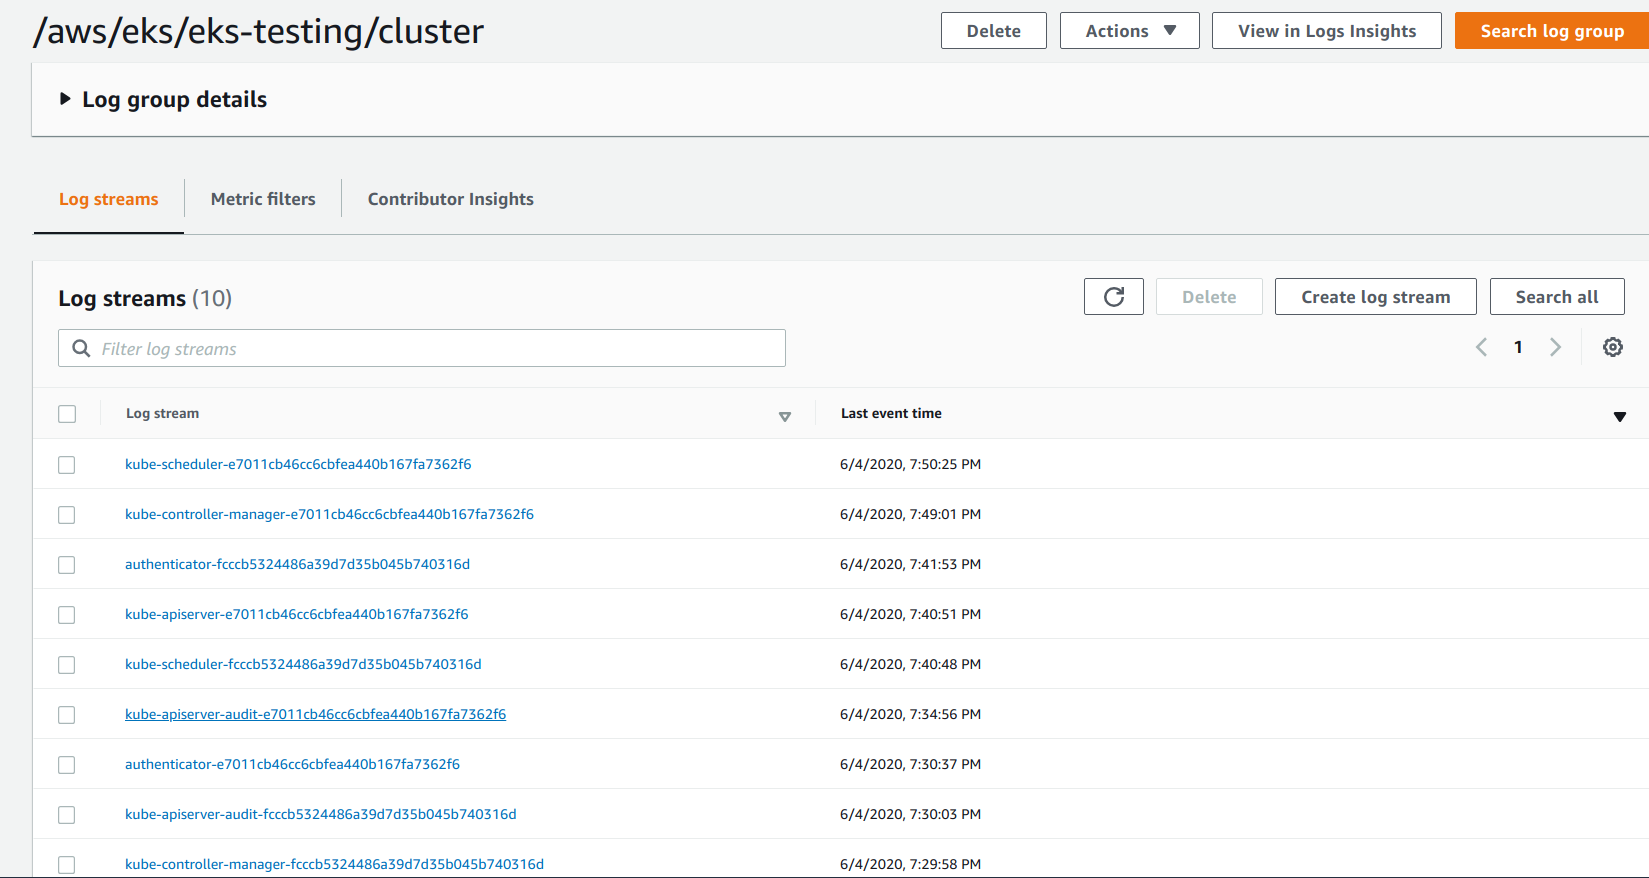
\includegraphics[width=16cm]{figures/eks-cw.png}
    \captionsetup{justification=centering,margin=2cm}
    \caption{CloudWatch logs for eksctl cluster}}
\end{figure}
\begin{figure}[H]
    \centering
    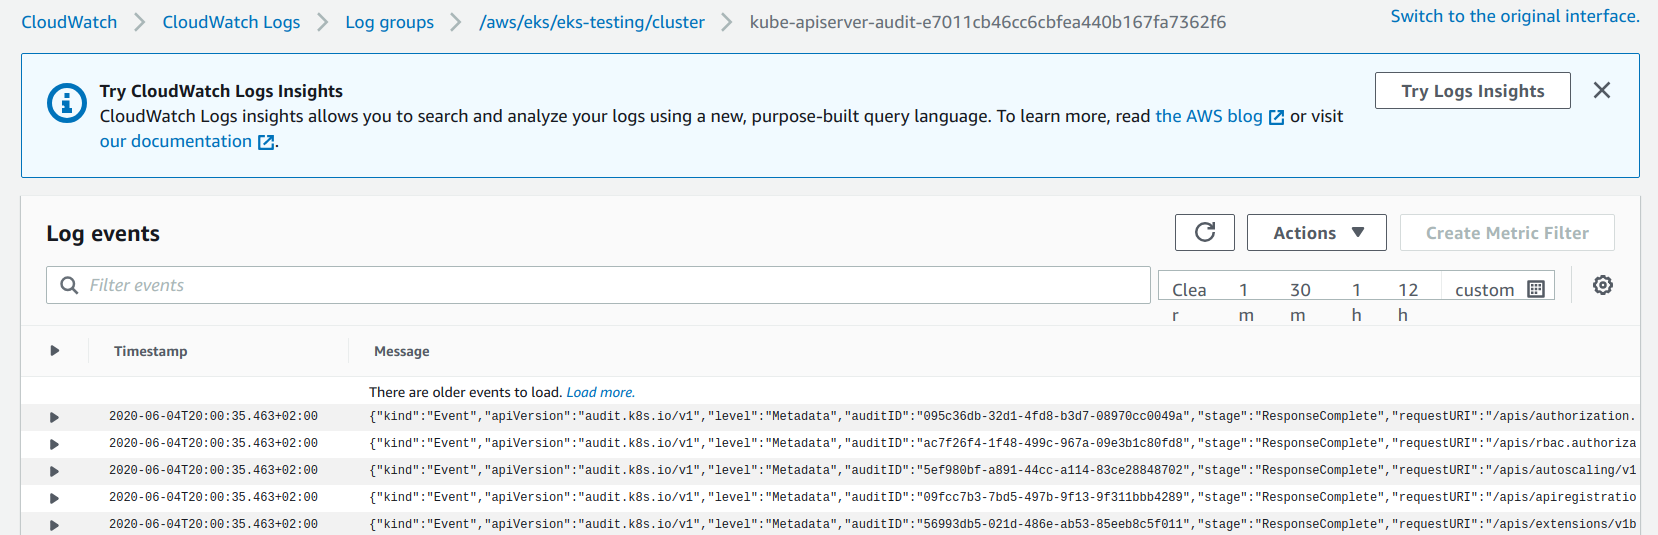
\includegraphics[width=16cm]{figures/eks-cw-apiserver.png}
    \captionsetup{justification=centering,margin=2cm}
    \caption{CloudWatch logs for eksctl cluster - concerning API server}}
\end{figure}

An example log message looked like this and it was in JSON format:

\begin{lstlisting}[basicstyle=\tiny,caption={Example log message},captionpos=b,language=Bash,xleftmargin=1cm]
2020-06-04T20:00:36.463+02:00
{
    "kind": "Event",
    "apiVersion": "audit.k8s.io/v1",
    "level": "Metadata",
    "auditID": "454b8586-2d17-4a53-9eb5-1e7422aabd21",
    "stage": "ResponseComplete",
    "requestURI": "/api?timeout=32s",
    "verb": "get",
    "user": {
        "username": "system:serviceaccount:kube-system:resourcequota-controller",
        "uid": "b7f3c725-196f-4b25-94e4-8f75614d3a04",
        "groups": [
            "system:serviceaccounts",
            "system:serviceaccounts:kube-system",
            "system:authenticated"
        ]
    },
    "sourceIPs": [
        "10.0.162.1"
    ],
    "userAgent": "kube-controller-manager/v1.16.8 (linux/amd64) \
      kubernetes/e163110/system:serviceaccount:kube-system:resourcequota-controller",
    "responseStatus": {
        "metadata": {},
        "code": 200
    },
    "requestReceivedTimestamp": "2020-06-04T18:00:36.279592Z",
    "stageTimestamp": "2020-06-04T18:00:36.279722Z",
    "annotations": {
        "authorization.k8s.io/decision": "allow",
        "authorization.k8s.io/reason": "RBAC: allowed by ClusterRoleBinding \
          \"system:discovery\" of ClusterRole \"system:discovery\" to Group \
          \"system:authenticated\""
    }
}
\end{lstlisting}

There was nothing needed to be done in order to provide High Availability. The control plane was already Highly Available because AWS EKS automatically provisions and scales the control plane across multiple AWS availability zones for high availability and fault tolerance\cite{eks-faqs}. Even the output provided when creating the cluster confirms the HA:
\begin{lstlisting}[basicstyle=\tiny,caption={Output from creating a eksctl cluster},captionpos=b,language=Bash,xleftmargin=1cm]
+ eksctl create cluster -f cluster.yaml
[ℹ]  eksctl version 0.20.0
[ℹ]  using region eu-west-1
[ℹ]  setting availability zones to [eu-west-1a eu-west-1b eu-west-1c]
[ℹ]  subnets for eu-west-1a - public:192.168.0.0/19 private:192.168.96.0/19
[ℹ]  subnets for eu-west-1b - public:192.168.32.0/19 private:192.168.128.0/19
[ℹ]  subnets for eu-west-1c - public:192.168.64.0/19 private:192.168.160.0/19
\end{lstlisting}

Central Monitoring system was also already available. AWS provides several metrics considering EC2 instances. The same metrics can be viewed in this section as in the according section for kops cluster. All the available metrics are presented in the following image.
\begin{figure}[H]
    \centering
    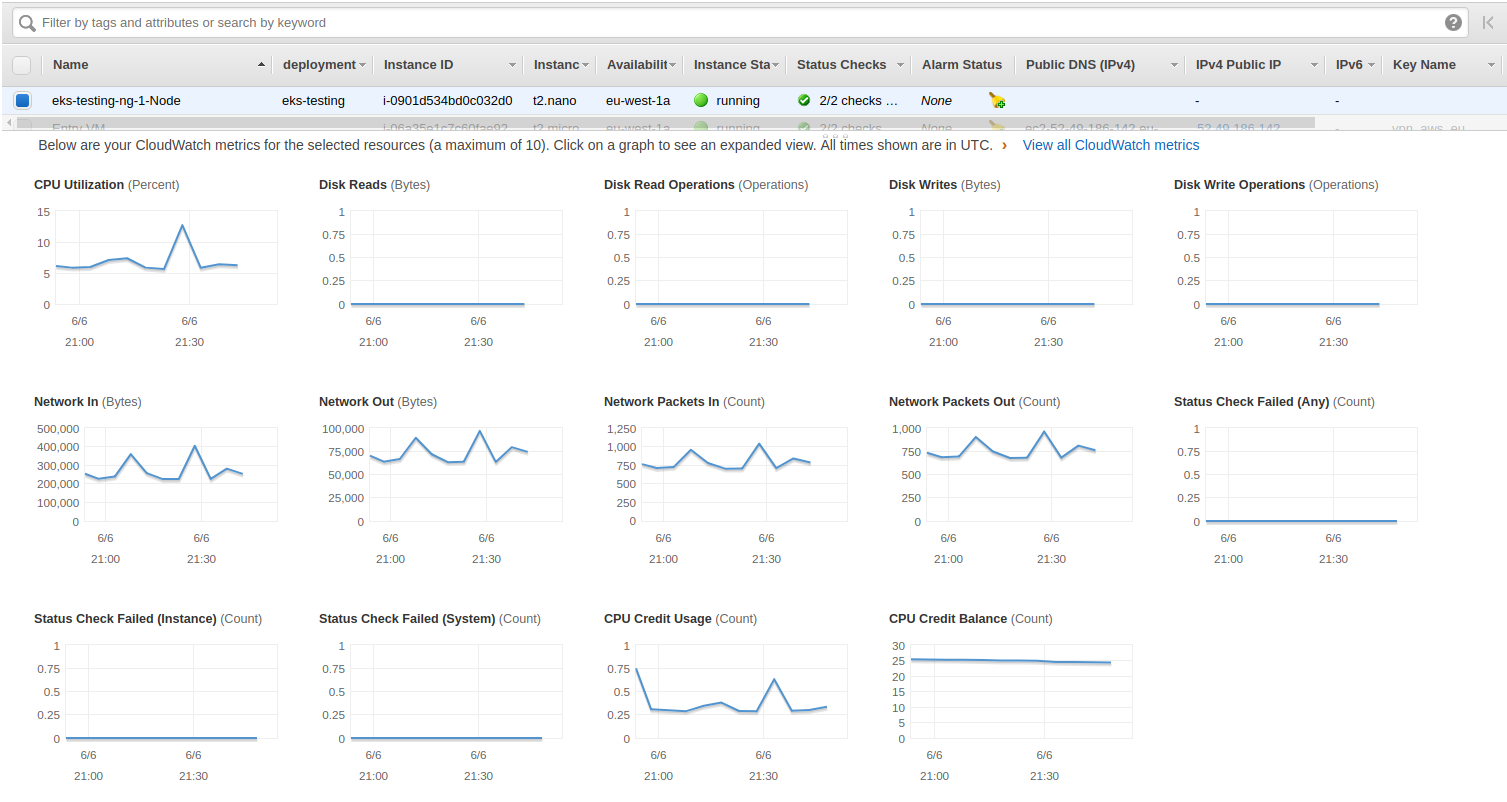
\includegraphics[width=17cm]{figures/eks-monitoring-ec2-node.png}
    \captionsetup{justification=centering,margin=2cm}
    \caption{CloudWatch monitoring for a worker node}
\end{figure}

When it comes to Central Audit, also no additional steps were taken. The actions performed on AWS resources are automatically visible on AWS CloudTrail dashboard. This is the same case as with kops. Since both methods use AWS, they both utilize CloudTrail. An example view showing the CloudTrail events, which occurred due to deleting an EKS cluster is shown next.
\begin{figure}[H]
    \centering
    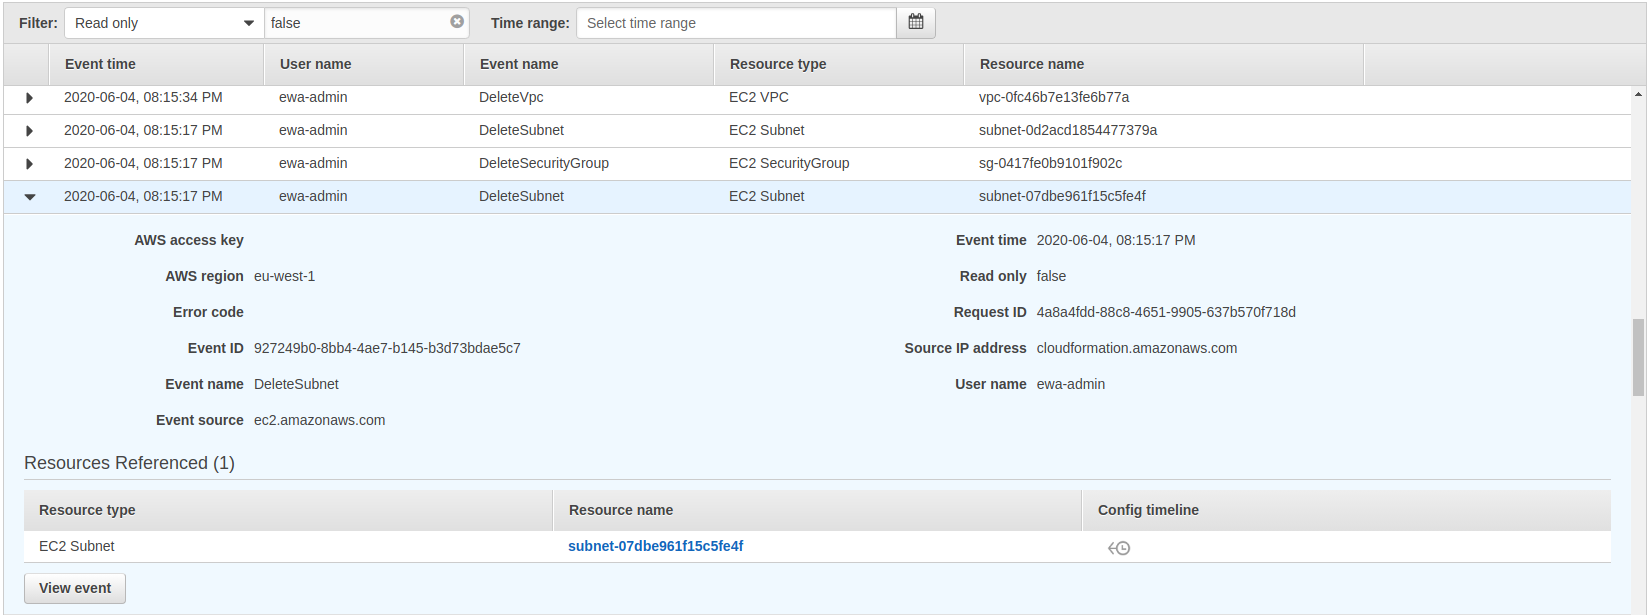
\includegraphics[width=17cm]{figures/eks-ct.png}
    \captionsetup{justification=centering,margin=2cm}
    \caption{CloudTrail events concerning eksctl cluster}}
\end{figure}

In order to make the cluster more secure, it was decided to restrict the ssh access and kubectl access. Searching through eksctl configuration, there was no setting which allowed to whitelist the IP addresses which are allowed to ssh login to worker nodes. However, blocking all the ssh access whatsover was available and it was chosen. This piece of code was needed to set that:
\begin{lstlisting}[basicstyle=\tiny,caption={Eksctl configuration applying security measures},captionpos=b,language=Bash,xleftmargin=1cm]
nodeGroups:
  - name: ng-1
    privateNetworking: true
    ssh:
      allow: false
\end{lstlisting}
This means now, that a cluster administrator has only kubectl access to cluster and no ssh access at all (because ssh access to worker nodes is blocked and access to master nodes is not given by design of AWS EKS). It is acknowledged that sometimes, not being able to ssh to the node may make troubleshooting more difficult, but generally system and EKS logs generally contain enough information for diagnosing problems. Usually the solution is to replace the problematic worker node rather than to diagnose and fix it\cite{eks-security}. Since no access to nodes is needed, thus also \textit{privateNetworking} under the \textit{nodeGroups} array was set to \textit{true}.

The second security requirement was to restrict the access to cluster through kubectl. By default, eksctl exposes the Kubernetes API server publicly but not directly from within the VPC subnets. This means that the public endpoint is by default set to true and the private endpoint to false\cite{eksctl-net}. In this work it was decided to apply the following configuration:
\begin{lstlisting}[basicstyle=\tiny,caption={Eksctl configuration applying security measures},captionpos=b,language=Bash,xleftmargin=1cm]
vpc:
  publicAccessCIDRs:
    - "<MY_PUBLIC_IP>/32"
  clusterEndpoints:
    publicAccess: true
    privateAccess: true
\end{lstlisting}
There were problems finding a working configuration, but it was finally solved thanks to a blog post\cite{eksctl-net-issue-solution} and thanks to eksctl official documentation\cite{eksctl-net}. The problems are described also in the section \ref{eks-troubleshooting}. The focal setting was \textit{publicAccessCIDRs}. It was set to the this-work-author's IP. Thus, only one IP address should be allowed to communicate with the cluster through kubectl. It was tested that the command kubectl worked from such an IP:
\begin{lstlisting}[basicstyle=\tiny,caption={Verifying connection to API server},captionpos=b,language=Bash,xleftmargin=1cm]
$ kubectl get nodes
NAME                                            STATUS   ROLES    AGE     VERSION
ip-192-168-126-229.eu-west-1.compute.internal   Ready    <none>   2m31s   v1.16.8-eks-e16311
\end{lstlisting}
and when the same command was run from a different machine, with a different IP, this command reached a timeout. Whenever there is a timeout when reaching an AWS endpoint, it may be caused by a Security Group not allowing such access. Thus, this proved that the kubectl access was restricted and, that security measures were working. Creating the EKS cluster with all the security settings took longer - about 25 minutes. But it was successful.

In order to meet the production deployment requirement of backup, Velero was used. The identical use case was tested as with the kops cluster. The result was identical, thus, there is no sense in describing it for the second time. Both: backup and restore operations went smoothly. But, one thing must be noted. An S3 bucket was needed as Velero backups destination. Thus, the bucket was created with:
\begin{lstlisting}[basicstyle=\tiny,caption={Creating an S3 bucket for Velero},captionpos=b,language=Bash,xleftmargin=1cm]
$ export K8S_EXP_VELERO_S3_BUCKET="k8s-eks-for-masters-thesis.k8s.local"
$ aws s3api create-bucket --bucket ${K8S_EXP_VELERO_S3_BUCKET} --region ${K8S_EXP_REGION} \
  --create-bucket-configuration LocationConstraint=${K8S_EXP_REGION}
$ aws s3api put-bucket-versioning --bucket ${K8S_EXP_VELERO_S3_BUCKET} \
  --versioning-configuration Status=Enabled
$ aws s3api put-bucket-encryption --bucket ${K8S_EXP_VELERO_S3_BUCKET} \
  --server-side-encryption-configuration '{"Rules":[{"ApplyServerSideEncryptionByDefault":{"SSEAlgorithm":"AES256"}}]}'
\end{lstlisting}
The backup created by Velero was put in the S3 bucket, which is presented on the illustration below:
\begin{figure}[H]
    \centering
    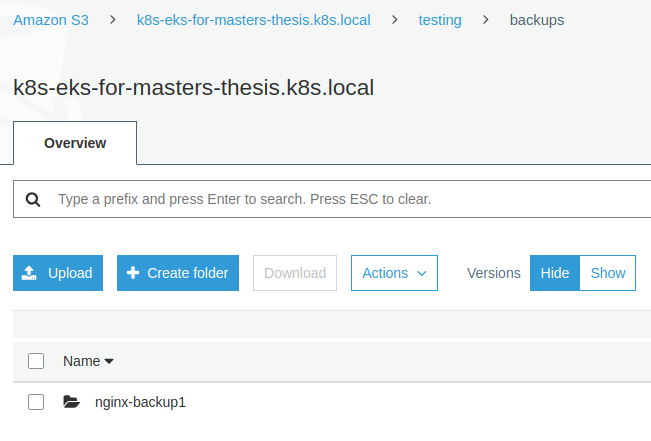
\includegraphics[width=14cm]{figures/eks-backup.png}
    \captionsetup{justification=centering,margin=2cm}
    \caption{Backup of eksctl cluster created by Velero}
\end{figure}

The next step was to deliver the autoscaling requirement. The same Kubernetes resources were used as with the kops method. This part of cluster configuration was needed to be put under the \textit{nodeGroups} YAML array:
\begin{lstlisting}[basicstyle=\tiny,caption={Eksctl configuration needed for autoscaler},captionpos=b,language=Bash,xleftmargin=1cm]
tags:
  # EC2 tags required for cluster-autoscaler auto-discovery
  k8s.io/cluster-autoscaler/enabled: "true"
  k8s.io/cluster-autoscaler/eks-testing: "owned"
iam:
  withAddonPolicies:
    autoScaler: true
    albIngress: true
    cloudWatch: true
\end{lstlisting}

Afterwards, the same procedure as described with kops was used. In result, deploying a test application and scaling its replicas number to 20 resulted in autoscaler adding another EC2 instance - a worker node. All the worker nodes were listed with the following commands:
\begin{lstlisting}[basicstyle=\tiny,caption={Listing EC2 instances, one was created by autoscaler},captionpos=b,language=Bash,xleftmargin=1cm]
eks$ aws ec2 describe-instances --filters "Name=tag-key,Values=deployment" --query "Reservations[*].Instances[*].{PublicIP:PublicIpAddress,Name:Tags[?Key=='Name']|[0].Value,Status:State.Name}"
[
    [
        {
            "PublicIP": null,
            "Name": "eks-testing-ng-1-Node",
            "Status": "running"
        }
    ],
    [
        {
            "PublicIP": null,
            "Name": "eks-testing-ng-1-Node",
            "Status": "running"
        }
    ]
]
eks$ kubectl get node
NAME                                            STATUS   ROLES    AGE   VERSION
ip-192-168-111-191.eu-west-1.compute.internal   Ready    <none>   67s   v1.16.8-eks-e16311
ip-192-168-162-84.eu-west-1.compute.internal    Ready    <none>   10m   v1.16.8-eks-e16311
\end{lstlisting}
Afterwards, the testing application was uninstalled with helm and after more than 5 minutes, the worker node EC2 instance was automatically removed.

\subsubsection{Testing a cluster}
The testing procedure was the same as with kops. Different command was invoked (because all the commands to run with eksctl were put into one file), but all the Bats-core tests were the same. Even the same bats files were used. There was obviously no \textit{kops validate cluster} command run, because that command was dedicated to kops clusters only. For the details, please refer to \ref{kops-testing}. Running all the tests took slightly less than 7 minutes. (It took long to have a working Load Balancer). The command to run tests was:
\begin{lstlisting}[basicstyle=\tiny,caption={Testing an eksctl cluster},captionpos=b,language=Bash,xleftmargin=1cm]
eks$ ./tasks _test
\end{lstlisting}

\subsubsection{Deleting a cluster}
In order to delete the cluster, one had to type:
\begin{lstlisting}[basicstyle=\tiny,caption={Deleting an eksctl cluster},captionpos=b,language=Bash,xleftmargin=1cm]
eks$ ./tasks _delete
\end{lstlisting}

This command usually took about 13 minutes. It deleted almost all AWS resources, but not CloudWatch LogGroup. Not deleting the LogGroup may be a good thing, because one may be interested to study the logs after the cluster is long gone. But still, it is good to know, that one has to delete it by themselves.

\subsubsection{Troubleshooting a cluster}
\label{eks-troubleshooting}

The same issues apply here, considering Velero, as with a cluster created with kops.


The greatest problem was how to set security measures. Setting the following in the YAML configuration file:
\begin{lstlisting}[basicstyle=\tiny,caption={Attempt to setup security},captionpos=b,language=Bash,xleftmargin=1cm]
vpc:
  publicAccessCIDRs:
    - "<MY_PUBLIC_IP>/32"
\end{lstlisting}
resulted in timeout on creating such cluster. It took 43 minutes then. The output ended with:

\begin{lstlisting}[basicstyle=\tiny,caption={Error output from creating eksctl cluster},captionpos=b,language=Bash,xleftmargin=1cm]
[ℹ]  adding identity "arn:aws:iam::976184668068:role/eksctl-eks-testing-nodegroup-ng-1-NodeInstanceRole-8VB5IDO1Z4KQ" to auth ConfigMap
[ℹ]  nodegroup "ng-1" has 0 node(s)
[ℹ]  waiting for at least 1 node(s) to become ready in "ng-1"
Error: timed out (after 25m0s) waiting for at least 1 nodes to join the cluster and become ready in "ng-1"
\end{lstlisting}
This problem was also acknowledged in eksctl Github.com issues\cite{eksctl-net-issue1}\cite{eksctl-net-issue2}. Even though the blog post\cite{eksctl-net-issue-solution}, which tremendously helped to find the working solution, suggested setting the following IAM policies to be configured under the \textit{nodeGroups} array, in practice, the IAM policies deemed unneeded. Cluster is working and healthy without them.
\begin{lstlisting}[basicstyle=\tiny,caption={IAM policies recommended for eksctl by a blog post},captionpos=b,language=Bash,xleftmargin=1cm]
nodeGroups:
    iam:
      attachPolicyARNs:
        - arn:aws:iam::aws:policy/AmazonEKSWorkerNodePolicy
        - arn:aws:iam::aws:policy/AmazonEKS_CNI_Policy
        - arn:aws:iam::aws:policy/ElasticLoadBalancingFullAccess
\end{lstlisting}

When deploying Cluster Autoscaler, there was a problem. The Cluster Autoscaler pod was in status: Pending. This is the same case as with the Velero Pod, described in \ref{kops-troubleshooting}. In this case there was too little memory. The EC2 instances type which was used initially, were \textit{t2.nano}. It was decided to try \textit{t2.micro} instances type. The problem was debugged with such commands:
\begin{lstlisting}[basicstyle=\tiny,caption={Debugging cluster autoscaler},captionpos=b,language=Bash,xleftmargin=1cm]
eks$ kubectl get -n kube-system pod
NAME                                  READY   STATUS    RESTARTS   AGE
aws-node-9sttv                        1/1     Running   0          61m
cluster-autoscaler-7d7b5564df-r6sqh   0/1     Pending   0          27s
coredns-8568c98b77-d7txg              0/1     Pending   0          74m
coredns-8568c98b77-hpmjk              1/1     Running   0          74m
kube-proxy-4qplq                      1/1     Running   0          61m
$ kubectl describe -n kube-system pod/cluster-autoscaler-7d7b5564df-r6sqh
# some output omitted
Events:
  Type     Reason            Age                From               Message
  ----     ------            ----               ----               -------
  Warning  FailedScheduling  66s (x2 over 66s)  default-scheduler  0/1 nodes are available: 1 Insufficient memory.
\end{lstlisting}

Using the \textit{t2.micro} instances type, there was a problem with deploying the test application:
\begin{lstlisting}[basicstyle=\tiny,caption={Debugging a test application},captionpos=b,language=Bash,xleftmargin=1cm]
$ kubectl -n testing describe pod/apache-testing-77594c54fb-fsc5s
# some output omitted
Events:
  Type     Reason            Age                 From               Message
  ----     ------            ----                ----               -------
  Warning  FailedScheduling  38s (x10 over 12m)  default-scheduler  0/1 nodes are available: 1 Insufficient pods.
\end{lstlisting}

The potential solution, found on Stack Overflow, suggested that \textit{t2.small} is the smallest instance type which is acceptable\cite{eks-instance-problem-so}. It turned out, that this problem was caused by an already described fact, that AWS EKS uses hard limits for number of pods allowed for a particular EC2 instance type\cite{eks-hard-limits}. Thus, even bigger instance was used: \textit{t2.small}. After the bigger instance type was used, all the pods in kube-system namespace were in status: Running.
\begin{lstlisting}[basicstyle=\tiny,caption={Verifying that all the pods are running},captionpos=b,language=Bash,xleftmargin=1cm]
eks$ kubectl get pod -n kube-system
NAME                       READY   STATUS    RESTARTS   AGE
aws-node-dk457             1/1     Running   0          3m38s
coredns-8568c98b77-gf5r4   1/1     Running   0          16m
coredns-8568c98b77-xg7jv   1/1     Running   0          16m
kube-proxy-hgjml           1/1     Running   0          3m38s
eks$ kubectl get pod -n testing
NAME                              READY   STATUS    RESTARTS   AGE
apache-testing-77594c54fb-nl5b2   1/1     Running   0          117s
\end{lstlisting}

Once, there was also a problem with deleting the EKS cluster. This was probably, because every time EKS was operated in the following way:
\begin{lstlisting}[basicstyle=\tiny,caption={Deleting eksctl cluster},captionpos=b,language=Bash,xleftmargin=1cm]
eks$ eksctl create cluster -f cluster.yaml
eks$ eksctl delete cluster -f cluster.yaml --wait
\end{lstlisting}
and this particular time, it was decided to delete a worker nodegroup with the intension to recreate it with different configuration. Therefore, this particular time, the cluster was operated in the following way and resulted in the following output:
\begin{lstlisting}[basicstyle=\tiny,caption={Eksctl special operations},captionpos=b,language=Bash,xleftmargin=1cm]
eks$ eksctl create cluster -f cluster.yaml
# output omitted
eks $ eksctl delete nodegroup -f cluster.yaml --approve
# some output omitted
[ℹ]  will delete stack "eksctl-eks-testing-nodegroup-ng-1"
[✔]  deleted 1 nodegroup(s) from cluster "eks-testing"
eks$ eksctl delete cluster -f cluster.yaml --wait
# some output omitted
[ℹ]  2 sequential tasks: { delete nodegroup "ng-1", delete cluster control plane "eks-testing" }
[ℹ]  will delete stack "eksctl-eks-testing-nodegroup-ng-1"
[ℹ]  waiting for stack "eksctl-eks-testing-nodegroup-ng-1" to get deleted
[✖]  unexpected status "DELETE_FAILED" while waiting for CloudFormation stack "eksctl-eks-testing-nodegroup-ng-1"
[ℹ]  fetching stack events in attempt to troubleshoot the root cause of the failure
[✖]  AWS::CloudFormation::Stack/eksctl-eks-testing-nodegroup-ng-1: DELETE_FAILED – "The following resource(s) failed to delete: [SG]. "
[✖]  AWS::EC2::SecurityGroup/SG: DELETE_FAILED – "resource sg-03f9a9928f765ecae has a dependent object (Service: AmazonEC2; Status Code: 400; Error Code: DependencyViolation; Request ID: 682fd971-5ec7-472e-9eee-4d52a44f9455)"
[ℹ]  1 error(s) occurred while deleting cluster with nodegroup(s)
[✖]  waiting for CloudFormation stack "eksctl-eks-testing-nodegroup-ng-1": ResourceNotReady: failed waiting for successful resource state
Error: failed to delete cluster with nodegroup(s)
\end{lstlisting}
Fortunately, running the \textit{eksctl delete cluster} again resulted in success.

\subsection{Troubleshooting any Kubernetes cluster}
\textit{This is a section dedicated to present the ideas of how to troubleshoot any Kubernetes cluster. The ideas were gathered during the empirical work of this study.}
\\

There are some general guidelines which help to debug the cluster. When a cluster is self-hosted and one is fully responsible for master and worker nodes deployment, then \textbf{one should verify whether any node is still functional}. It means that problems like: corrupt filesystem, kernel deadlock, problems with the Docker Daemon or problems with hardware may occur and should be mitigated. A solution to detect such problems may be: a node problem detector pod\cite{book-mastering-k8s}. One should also run the following commands to check if all the worker nodes are running and if the cluster is generally reachable. But, since this work focuses on deployments on the cloud, then the problems described in this paragraph should be already taken care of.
\begin{lstlisting}[basicstyle=\tiny,caption={Getting information about a cluster},captionpos=b,language=Bash,xleftmargin=1cm]
$ kubectl get nodes
$ kubectl cluster-info
\end{lstlisting}

Another level of troubleshooting is \textbf{debugging the applications deployed on top of the Kubernetes cluster}. Some ideas are discribed on the official Kubernetes documentation website\cite{k8s-deb}. For example, one can get details of a pod with the following commands:
\begin{lstlisting}[basicstyle=\tiny,caption={Getting information about pods},captionpos=b,language=Bash,xleftmargin=1cm]
$ kubectl describe pods ${POD_NAME}
$ kubectl logs ${POD_NAME}
\end{lstlisting}

Even the \textbf{pod status} may provide us with enough information, what steps should be taken next. If a pod is in Pending status, then it could mean that there are not enough resources in the cluster (e.g. the worker nodes use too small EC2 instance types or there are too few worker nodes). A pod may be also in status CrashLoopBackOff which indicates that a container is repeatedly crashing after restarting. There may a problem also that a Docker image for a container cannot be downloaded and a pod may be in state ImagePullBackOff or ErrImagePull\cite{k8s-google-tr}.

It is also always a good idea to \textbf{read log messages} (so access to log messages should be always supplied). The following Kubernetes components log messages may be helpful\cite{k8s-deb-cluster}:
\begin{itemize}
\item logs from kube-apiserver - which is responsible for serving the API
\item logs from kube-scheduler - which is responsible for making scheduling decisions
\item logs from kube-controller-manager - which manages replication controllers
\item logs from kubelet - which is responsible for running containers on the node
\item logs from kube-proxy - which is responsible for service load balancing
\end{itemize}

Besides all the troubleshooting ideas presented earlier, one can also visit solutions dedicated entirely to AWS EKS clusters\cite{k8s-eks-tr} or to eksctl\cite{k8s-eksctl-tr}. Still, some problems may be tough to handle. But even then, there are always measures that could be applied to move further into the correct direction. One may \textbf{ask a question} on Stack Overflow or talk to a Kubernetes team on Slack or write on a Kubernetes forum or file a bug on Kubernetes Github.com project website\cite{k8s-deb-ask}.

To summarize: there are various ways how to debug a Kubernetes cluster or an application deployed on top of it. Some steps may be applied to any Kubernetes cluster, other concern only the clusters deployed using a particular method. Nevertheless, if one is in need, they can ask for help or talk with people who are more experienced with Kubernetes.
